\documentclass[a4paper,11pt]{article}

% Essential Packages
\usepackage{graphicx}       % For importing images
\usepackage{geometry}       % For page margins
\usepackage{booktabs}       % For professional looking tables
\usepackage{amsmath}        % For math formatting
\usepackage{float}          % To control figure placement
\usepackage[utf8]{inputenc}
\usepackage{caption}        % For better caption control
\usepackage{hyperref}       % For clickable links (optional)
\usepackage{subcaption}


% Page Layout Setup
\geometry{margin=1in}

% ============================================================
% IMAGE / PLOT PATH MAPPING -- place these files before compiling.
% Every \includegraphics path below is images/... or plots/..., matching
% main_dr.tex's convention. Nothing under images/ or plots/ is created by
% this commit -- copy each source file (already produced by eigen_analysis.py
% and recon_images.py) to the listed target path.
%
% -- OD_256 --
%   plots/OD_256_RawMoments_beta_0.01.png  <-  saved_matrices/OD_256/RawMoments_beta_0.01.png
%   plots/OD_256_Covariance_beta_0.01.png  <-  saved_matrices/OD_256/Covariance_beta_0.01.png
%   plots/OD_256_Correlation_beta_0.01.png  <-  saved_matrices/OD_256/Correlation_beta_0.01.png
%   plots/OD_256_FrobeniusNormSquared_RawMoments.png  <-  saved_matrices/OD_256/FrobeniusNormSquared_RawMoments.png
%   plots/OD_256_FrobeniusNormSquared_Covariance.png  <-  saved_matrices/OD_256/FrobeniusNormSquared_Covariance.png
%   plots/OD_256_FrobeniusNormSquared_Correlation.png  <-  saved_matrices/OD_256/FrobeniusNormSquared_Correlation.png
%   images/OD_256_original_0.png  <-  original_OD_256/orig_00000.png
%   images/OD_256_original_1.png  <-  original_OD_256/orig_00001.png
%   images/OD_256_original_2.png  <-  original_OD_256/orig_00002.png
%   images/OD_256_original_3.png  <-  original_OD_256/orig_00003.png
%   images/OD_256_original_4.png  <-  original_OD_256/orig_00004.png
%   images/OD_256_recon_cor_0_beta_99.png  <-  reconstructed_OD_256_cor/recon_cor_00000.png
%   images/OD_256_recon_cor_1_beta_99.png  <-  reconstructed_OD_256_cor/recon_cor_00001.png
%   images/OD_256_recon_cor_2_beta_99.png  <-  reconstructed_OD_256_cor/recon_cor_00002.png
%   images/OD_256_recon_cor_3_beta_99.png  <-  reconstructed_OD_256_cor/recon_cor_00003.png
%   images/OD_256_recon_cor_4_beta_99.png  <-  reconstructed_OD_256_cor/recon_cor_00004.png
%   images/OD_256_recon_cor_0_beta_95.png  <-  reconstructed_OD_256_cor_95/recon_cor_00000.png
%   images/OD_256_recon_cor_1_beta_95.png  <-  reconstructed_OD_256_cor_95/recon_cor_00001.png
%   images/OD_256_recon_cor_2_beta_95.png  <-  reconstructed_OD_256_cor_95/recon_cor_00002.png
%   images/OD_256_recon_cor_3_beta_95.png  <-  reconstructed_OD_256_cor_95/recon_cor_00003.png
%   images/OD_256_recon_cor_4_beta_95.png  <-  reconstructed_OD_256_cor_95/recon_cor_00004.png
%   images/OD_256_recon_cor_0_beta_90.png  <-  reconstructed_OD_256_cor_90/recon_cor_00000.png
%   images/OD_256_recon_cor_1_beta_90.png  <-  reconstructed_OD_256_cor_90/recon_cor_00001.png
%   images/OD_256_recon_cor_2_beta_90.png  <-  reconstructed_OD_256_cor_90/recon_cor_00002.png
%   images/OD_256_recon_cor_3_beta_90.png  <-  reconstructed_OD_256_cor_90/recon_cor_00003.png
%   images/OD_256_recon_cor_4_beta_90.png  <-  reconstructed_OD_256_cor_90/recon_cor_00004.png
% -- OD_512 --
%   plots/OD_512_RawMoments_beta_0.01.png  <-  saved_matrices/OD_512/RawMoments_beta_0.01.png
%   plots/OD_512_Covariance_beta_0.01.png  <-  saved_matrices/OD_512/Covariance_beta_0.01.png
%   plots/OD_512_Correlation_beta_0.01.png  <-  saved_matrices/OD_512/Correlation_beta_0.01.png
%   plots/OD_512_FrobeniusNormSquared_RawMoments.png  <-  saved_matrices/OD_512/FrobeniusNormSquared_RawMoments.png
%   plots/OD_512_FrobeniusNormSquared_Covariance.png  <-  saved_matrices/OD_512/FrobeniusNormSquared_Covariance.png
%   plots/OD_512_FrobeniusNormSquared_Correlation.png  <-  saved_matrices/OD_512/FrobeniusNormSquared_Correlation.png
%   images/OD_512_original_0.png  <-  original_OD_512/orig_00000.png
%   images/OD_512_original_1.png  <-  original_OD_512/orig_00001.png
%   images/OD_512_original_2.png  <-  original_OD_512/orig_00002.png
%   images/OD_512_original_3.png  <-  original_OD_512/orig_00003.png
%   images/OD_512_original_4.png  <-  original_OD_512/orig_00004.png
%   images/OD_512_recon_cor_0_beta_99.png  <-  reconstructed_OD_512_cor/recon_cor_00000.png
%   images/OD_512_recon_cor_1_beta_99.png  <-  reconstructed_OD_512_cor/recon_cor_00001.png
%   images/OD_512_recon_cor_2_beta_99.png  <-  reconstructed_OD_512_cor/recon_cor_00002.png
%   images/OD_512_recon_cor_3_beta_99.png  <-  reconstructed_OD_512_cor/recon_cor_00003.png
%   images/OD_512_recon_cor_4_beta_99.png  <-  reconstructed_OD_512_cor/recon_cor_00004.png
%   images/OD_512_recon_cor_0_beta_95.png  <-  reconstructed_OD_512_cor_95/recon_cor_00000.png
%   images/OD_512_recon_cor_1_beta_95.png  <-  reconstructed_OD_512_cor_95/recon_cor_00001.png
%   images/OD_512_recon_cor_2_beta_95.png  <-  reconstructed_OD_512_cor_95/recon_cor_00002.png
%   images/OD_512_recon_cor_3_beta_95.png  <-  reconstructed_OD_512_cor_95/recon_cor_00003.png
%   images/OD_512_recon_cor_4_beta_95.png  <-  reconstructed_OD_512_cor_95/recon_cor_00004.png
%   images/OD_512_recon_cor_0_beta_90.png  <-  reconstructed_OD_512_cor_90/recon_cor_00000.png
%   images/OD_512_recon_cor_1_beta_90.png  <-  reconstructed_OD_512_cor_90/recon_cor_00001.png
%   images/OD_512_recon_cor_2_beta_90.png  <-  reconstructed_OD_512_cor_90/recon_cor_00002.png
%   images/OD_512_recon_cor_3_beta_90.png  <-  reconstructed_OD_512_cor_90/recon_cor_00003.png
%   images/OD_512_recon_cor_4_beta_90.png  <-  reconstructed_OD_512_cor_90/recon_cor_00004.png
% -- FOVEA_256 --
%   plots/FOVEA_256_RawMoments_beta_0.01.png  <-  saved_matrices/FOVEA_256/RawMoments_beta_0.01.png
%   plots/FOVEA_256_Covariance_beta_0.01.png  <-  saved_matrices/FOVEA_256/Covariance_beta_0.01.png
%   plots/FOVEA_256_Correlation_beta_0.01.png  <-  saved_matrices/FOVEA_256/Correlation_beta_0.01.png
%   plots/FOVEA_256_FrobeniusNormSquared_RawMoments.png  <-  saved_matrices/FOVEA_256/FrobeniusNormSquared_RawMoments.png
%   plots/FOVEA_256_FrobeniusNormSquared_Covariance.png  <-  saved_matrices/FOVEA_256/FrobeniusNormSquared_Covariance.png
%   plots/FOVEA_256_FrobeniusNormSquared_Correlation.png  <-  saved_matrices/FOVEA_256/FrobeniusNormSquared_Correlation.png
%   images/FOVEA_256_original_0.png  <-  original_FOVEA_256/orig_00000.png
%   images/FOVEA_256_original_1.png  <-  original_FOVEA_256/orig_00001.png
%   images/FOVEA_256_original_2.png  <-  original_FOVEA_256/orig_00002.png
%   images/FOVEA_256_original_3.png  <-  original_FOVEA_256/orig_00003.png
%   images/FOVEA_256_original_4.png  <-  original_FOVEA_256/orig_00004.png
%   images/FOVEA_256_recon_cor_0_beta_99.png  <-  reconstructed_FOVEA_256_cor/recon_cor_00000.png
%   images/FOVEA_256_recon_cor_1_beta_99.png  <-  reconstructed_FOVEA_256_cor/recon_cor_00001.png
%   images/FOVEA_256_recon_cor_2_beta_99.png  <-  reconstructed_FOVEA_256_cor/recon_cor_00002.png
%   images/FOVEA_256_recon_cor_3_beta_99.png  <-  reconstructed_FOVEA_256_cor/recon_cor_00003.png
%   images/FOVEA_256_recon_cor_4_beta_99.png  <-  reconstructed_FOVEA_256_cor/recon_cor_00004.png
%   images/FOVEA_256_recon_cor_0_beta_95.png  <-  reconstructed_FOVEA_256_cor_95/recon_cor_00000.png
%   images/FOVEA_256_recon_cor_1_beta_95.png  <-  reconstructed_FOVEA_256_cor_95/recon_cor_00001.png
%   images/FOVEA_256_recon_cor_2_beta_95.png  <-  reconstructed_FOVEA_256_cor_95/recon_cor_00002.png
%   images/FOVEA_256_recon_cor_3_beta_95.png  <-  reconstructed_FOVEA_256_cor_95/recon_cor_00003.png
%   images/FOVEA_256_recon_cor_4_beta_95.png  <-  reconstructed_FOVEA_256_cor_95/recon_cor_00004.png
%   images/FOVEA_256_recon_cor_0_beta_90.png  <-  reconstructed_FOVEA_256_cor_90/recon_cor_00000.png
%   images/FOVEA_256_recon_cor_1_beta_90.png  <-  reconstructed_FOVEA_256_cor_90/recon_cor_00001.png
%   images/FOVEA_256_recon_cor_2_beta_90.png  <-  reconstructed_FOVEA_256_cor_90/recon_cor_00002.png
%   images/FOVEA_256_recon_cor_3_beta_90.png  <-  reconstructed_FOVEA_256_cor_90/recon_cor_00003.png
%   images/FOVEA_256_recon_cor_4_beta_90.png  <-  reconstructed_FOVEA_256_cor_90/recon_cor_00004.png
% -- FOVEA_512 --
%   plots/FOVEA_512_RawMoments_beta_0.01.png  <-  saved_matrices/FOVEA_512/RawMoments_beta_0.01.png
%   plots/FOVEA_512_Covariance_beta_0.01.png  <-  saved_matrices/FOVEA_512/Covariance_beta_0.01.png
%   plots/FOVEA_512_Correlation_beta_0.01.png  <-  saved_matrices/FOVEA_512/Correlation_beta_0.01.png
%   plots/FOVEA_512_FrobeniusNormSquared_RawMoments.png  <-  saved_matrices/FOVEA_512/FrobeniusNormSquared_RawMoments.png
%   plots/FOVEA_512_FrobeniusNormSquared_Covariance.png  <-  saved_matrices/FOVEA_512/FrobeniusNormSquared_Covariance.png
%   plots/FOVEA_512_FrobeniusNormSquared_Correlation.png  <-  saved_matrices/FOVEA_512/FrobeniusNormSquared_Correlation.png
%   images/FOVEA_512_original_0.png  <-  original_FOVEA_512/orig_00000.png
%   images/FOVEA_512_original_1.png  <-  original_FOVEA_512/orig_00001.png
%   images/FOVEA_512_original_2.png  <-  original_FOVEA_512/orig_00002.png
%   images/FOVEA_512_original_3.png  <-  original_FOVEA_512/orig_00003.png
%   images/FOVEA_512_original_4.png  <-  original_FOVEA_512/orig_00004.png
%   images/FOVEA_512_recon_cor_0_beta_99.png  <-  reconstructed_FOVEA_512_cor/recon_cor_00000.png
%   images/FOVEA_512_recon_cor_1_beta_99.png  <-  reconstructed_FOVEA_512_cor/recon_cor_00001.png
%   images/FOVEA_512_recon_cor_2_beta_99.png  <-  reconstructed_FOVEA_512_cor/recon_cor_00002.png
%   images/FOVEA_512_recon_cor_3_beta_99.png  <-  reconstructed_FOVEA_512_cor/recon_cor_00003.png
%   images/FOVEA_512_recon_cor_4_beta_99.png  <-  reconstructed_FOVEA_512_cor/recon_cor_00004.png
%   images/FOVEA_512_recon_cor_0_beta_95.png  <-  reconstructed_FOVEA_512_cor_95/recon_cor_00000.png
%   images/FOVEA_512_recon_cor_1_beta_95.png  <-  reconstructed_FOVEA_512_cor_95/recon_cor_00001.png
%   images/FOVEA_512_recon_cor_2_beta_95.png  <-  reconstructed_FOVEA_512_cor_95/recon_cor_00002.png
%   images/FOVEA_512_recon_cor_3_beta_95.png  <-  reconstructed_FOVEA_512_cor_95/recon_cor_00003.png
%   images/FOVEA_512_recon_cor_4_beta_95.png  <-  reconstructed_FOVEA_512_cor_95/recon_cor_00004.png
%   images/FOVEA_512_recon_cor_0_beta_90.png  <-  reconstructed_FOVEA_512_cor_90/recon_cor_00000.png
%   images/FOVEA_512_recon_cor_1_beta_90.png  <-  reconstructed_FOVEA_512_cor_90/recon_cor_00001.png
%   images/FOVEA_512_recon_cor_2_beta_90.png  <-  reconstructed_FOVEA_512_cor_90/recon_cor_00002.png
%   images/FOVEA_512_recon_cor_3_beta_90.png  <-  reconstructed_FOVEA_512_cor_90/recon_cor_00003.png
%   images/FOVEA_512_recon_cor_4_beta_90.png  <-  reconstructed_FOVEA_512_cor_90/recon_cor_00004.png
% ============================================================

% Title Information
\title{\textbf{Dimension Reduction Analysis Report: Region Crops (Optic Disc \& Fovea)}}
\date{September 15, 2026}

\begin{document}

\maketitle

\section{Objective}
Whole fundus images spend most of their dimensionality on padding,
background, and anatomy that is not diagnostically relevant. The objective
of this analysis is to instead extract two clinically relevant regions from
every MESSIDOR image -- the \textbf{Optic Disc (OD)} and the \textbf{Fovea
(FOVEA)} -- using pixel coordinates derived from vascX segmentations, and
perform dimension reduction (Raw Moments, Covariance, Correlation)
independently on each region at two crop sizes, $s \in \{256, 512\}$. We
then reconstruct every crop from its truncated basis and quantify the
reconstruction quality directly in pixel space via Mean Squared Error (MSE),
for $\beta \in \{0.01, 0.05, 0.10\}$.

\section{Methodology}

\subsection{Coordinate-Based Region Extraction}
For every image we are given optic disc and fovea center coordinates
$(od_x,od_y)$ and $(fovea_x,fovea_y)$, obtained from vascX segmentations of
each fundus image and stored in \texttt{messidor\_od\_fovea.csv}. For a crop size $s$,
a square window of size $s\times s$ is extracted centered on each coordinate;
if the window would run off the edge of the image it is shifted inward
(rather than padded) so that it stays fully inside the source image --
padding with black pixels only occurs if the source image itself is smaller
than $s$ in that dimension. Each crop is flattened into a vector
$h_i^{OD}, h_i^{FOVEA} \in \mathbb{R}^d$ with $d = 3s^2$, giving Data
Matrices $H^{OD}_{s}$ and $H^{FOVEA}_{s}$ of shape $(d, 1745)$ for each
$s \in \{256, 512\}$ -- four independent crop configurations in total.

\subsection{Space-Efficient $H^TH$ Construction}
Due to the size of each crop, $H^TH$ is built without ever holding the full
Data Matrix $H$ in memory, using
$(H^TH)_{i:i+l,j:j+l} = (H_{i:i+l})^TH_{j:j+l}$ over batches of $l$ images
at a time. This is repeated independently for each of the four
$(region, size)$ configurations, producing $H^TH_{region,size}$
($1745\times1745$), together with the mean vector $\mu_{region,size}$ and
standard-deviation vector $\sigma_{region,size}$.

\subsubsection{Covariance Matrix Calculation}
Let $\mathbf{1}$ be a column vector of ones of length $n=1745$, and let
$\mu$ be the mean crop vector. Centering each column of $H$ by $\mu$ before
forming $H^TH$ gives:
\begin{align*}
    H^TH_{Covariance} &= \frac{1}{n}(H-\mu\mathbf{1}^T)^T(H-\mu\mathbf{1}^T)\\
    &= \frac{1}{n}(H^T-\mathbf{1}\mu^T)(H-\mu\mathbf{1}^T)\\
    &= \frac{1}{n}(H^TH+\mathbf{1}\mu^T\mu\mathbf{1}^T-\mathbf{1}\mu^TH-H^T\mu\mathbf{1}^T)
\end{align*}
Since $\mu = \frac{1}{n}H\mathbf{1}$, the cross terms $\mathbf{1}\mu^TH$ and
$H^T\mu\mathbf{1}^T$ can be rewritten purely in terms of $H^TH$:
\begin{align*}
    H^TH_{Covariance} &= \frac{1}{n}\left(H^TH+\mathbf{1}\mu^T\mu\mathbf{1}^T-\mathbf{1}\left(\frac{1}{n}H\mathbf{1}\right)^TH-H^T\left(\frac{1}{n}H\mathbf{1}\right)\mathbf{1}^T\right)\\
    &= \frac{1}{n}\left(H^TH + \mathbf{1}\mu^T\mu\mathbf{1}^T - \frac{1}{n}\mathbf{1}\mathbf{1}^T(H^TH) - \frac{1}{n}(H^TH)\mathbf{1}\mathbf{1}^T\right)
\end{align*}
so $H^TH_{Covariance}$ is computable from $H^TH$ and $\mu$ alone, without
ever recentering $H$ or recomputing pairwise dot products.

\subsubsection{Correlation Matrix Calculation}
Let $\Sigma_- = diag(1/\sigma_i)$, so that right-multiplying the centered
data by $\Sigma_-$ standardizes each row to unit variance. Then:
\begin{align*}
    H^TH_{Correlation} &= \frac{1}{n}\big((H-\mu\mathbf{1}^T)\Sigma_-\big)^T\big((H-\mu\mathbf{1}^T)\Sigma_-\big)\\
    &= \frac{1}{n}\Sigma_-^T(H-\mu\mathbf{1}^T)^T(H-\mu\mathbf{1}^T)\Sigma_-\\
    &= \Sigma_-^TH^TH_{Covariance}\Sigma_-
\end{align*}
so the correlation form follows directly from the covariance form above by
a diagonal rescaling, again with no further pass over the images.

\subsection{Component Selection}
Let $H = U\Sigma V^T$ be the singular value decomposition of a (variant of
the) Data Matrix $H$, so that $H^TH = V\Sigma^2V^T$ is exactly the
eigendecomposition computed above, with eigenvalues $\Sigma^2$ and
eigenvectors $V$. Partitioning $U$, $\Sigma$, $V$ into a kept block (subscript
$1$, the top $k$ components) and a discarded block (subscript $2$),
\begin{displaymath}
    (U_1^TH)_{k\times n} = \Sigma_1^{\frac{1}{2}}V_1^T,
\end{displaymath}
i.e.\ the reduced Data Matrix is exactly the top-$k$ singular values scaled
into the top-$k$ right-singular vectors. For each $(region, size, variant)$
combination we eigendecompose the corresponding $H^TH$ and pick the
smallest $k$ whose cumulative eigenvalue sum reaches $1-\beta$ of the total.
The quality of this truncation is measured by the Frobenius norm error of
the discarded block,
\begin{displaymath}
    F_{err} = Tr(\Sigma_2^2) = \sum_{\text{discarded }i}\lambda_i,
\end{displaymath}
i.e. the sum of the eigenvalues \emph{not} kept.

\subsection{Reconstruction}
From the SVD, the best rank-$k$ reconstruction of $H$ is
\begin{displaymath}
    \hat H = U_1\Sigma_1^{\frac{1}{2}}V_1^T = U_1U_1^TH.
\end{displaymath}
Computing $U_1$ directly would require eigendecomposing $HH^T$, a
$d\times d$ matrix (up to $786432\times786432$ for $s=512$ crops) -- far too
large to hold in memory. Instead, using $U_1 = HV_1\Sigma_1^{-\frac{1}{2}}$
(which follows from $H = U\Sigma V^T \Rightarrow HV_1 = U_1\Sigma_1$):
\begin{align*}
    \hat H &= U_1\Sigma_1^{\frac{1}{2}}V_1^T\\
    &= \left(HV_1\Sigma_1^{-\frac{1}{2}}\right)\Sigma_1^{\frac{1}{2}}V_1^T\\
    &= HV_1V_1^T,
\end{align*}
applied independently to each crop's Data Matrix and its own top-$k$
eigenvectors $V_1$.

\subsection{Reconstruction Quality: Mean Squared Error}
In addition to the analytic Frobenius-norm error above, we report the
pixel-space Mean Squared Error between every crop and its reconstruction,
\begin{displaymath}
    MSE = \frac{1}{nd}\sum_{i=1}^{n} \lVert h_i - \hat h_i \rVert_2^2,
\end{displaymath}
computed over all $n=1745$ crops for each $(region, size, variant, \beta)$
combination, with $\beta \in \{0.01, 0.05, 0.10\}$. Only 5 representative
original/reconstructed pairs per configuration are saved to disk for visual
inspection; the MSE itself is computed over the full set of 1745 images.

\section{Results}

% ============================================================
% OD 256
% ============================================================

\subsection{Optic Disc, $256\times256$}

\begin{table}[H]
    \centering
    \caption{Component Selection Summary -- OD, $s=256$}
    \label{tab:results_od_256}
    \vspace{0.2cm}
    \begin{tabular}{lrrrrr}
        \toprule
        \textbf{Analysis Type} & \textbf{$\beta$} & \textbf{Cutoff} & \textbf{Components Kept ($k$)} & \textbf{Actual Var. Expl.} & \textbf{Frobenius Norm} \\
        \midrule
        Raw Moments & 0.01 & 99.00\% & \textbf{5} & 99.06\% & 891832.85\\
        Covariance  & 0.01 & 99.00\% & \textbf{593} & 99.00\% & 28.46 \\
        Correlation  & 0.01 & 99.00\% & \textbf{701} & 99.00\% & 0.01\\
        \bottomrule
    \end{tabular}
\end{table}

\begin{figure}[H]
    \centering
    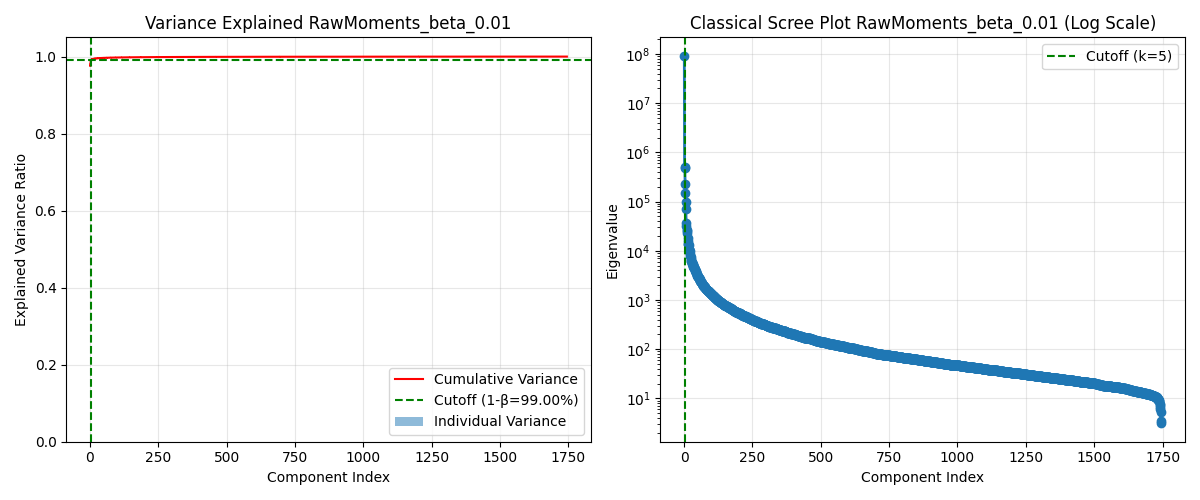
\includegraphics[width=\textwidth]{plots/OD_256_RawMoments_beta_0.01.png}
    \caption{\textbf{Raw Moments Analysis, OD $256\times256$.} Scree plot and explained variance for $\beta=0.01$, requiring $k=5$ components.}
    \label{fig:od256_raw}
\end{figure}

\begin{figure}[H]
    \centering
    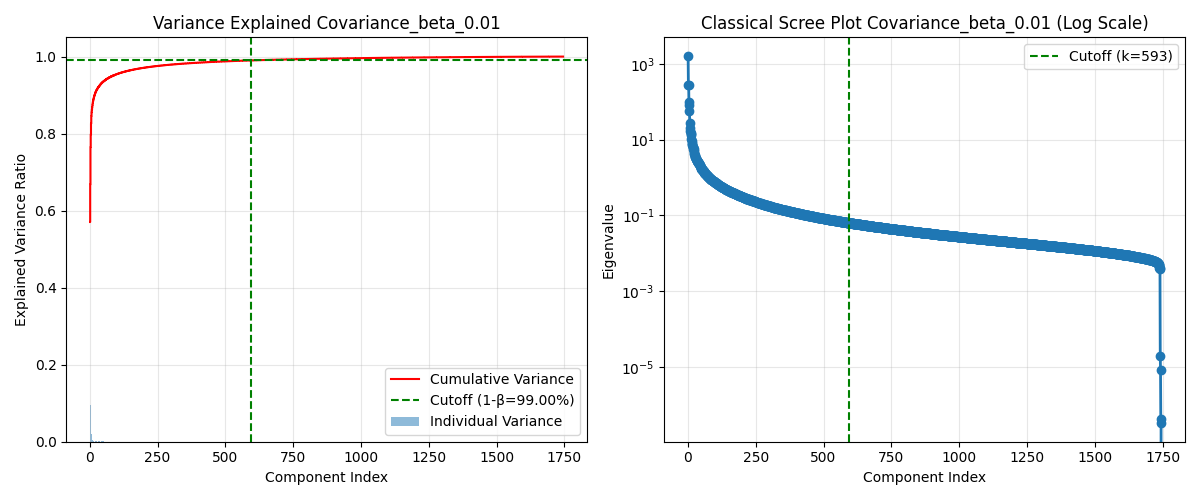
\includegraphics[width=\textwidth]{plots/OD_256_Covariance_beta_0.01.png}
    \caption{\textbf{Covariance Analysis (PCA), OD $256\times256$.} Requires $k=593$ components to meet the $\beta=0.01$ threshold.}
    \label{fig:od256_cov}
\end{figure}

\begin{figure}[H]
    \centering
    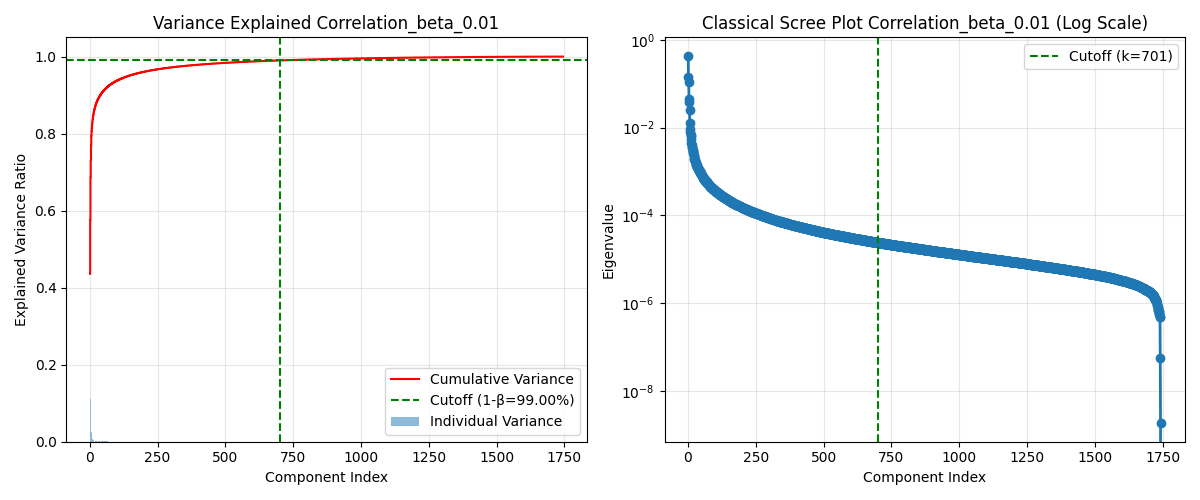
\includegraphics[width=\textwidth]{plots/OD_256_Correlation_beta_0.01.png}
    \caption{\textbf{Correlation Analysis, OD $256\times256$.} Requires $k=701$ components.}
    \label{fig:od256_cor}
\end{figure}

\begin{figure}[H]
    \centering
    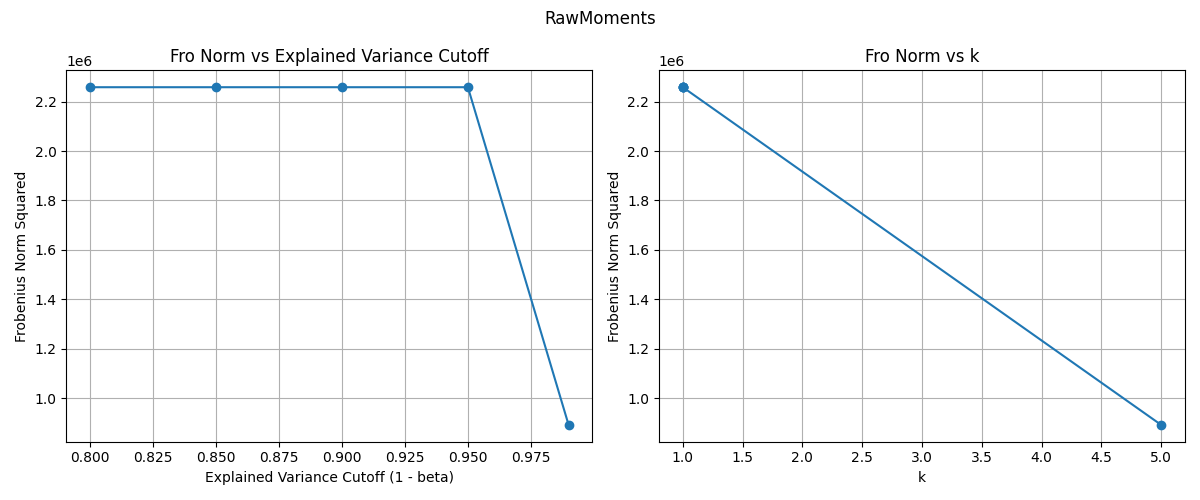
\includegraphics[width=\textwidth]{plots/OD_256_FrobeniusNormSquared_RawMoments.png}
    \caption{\textbf{Frobenius Norm Squared vs $\beta$, OD $256\times256$, Raw Moments.}}
    \label{fig:fronorm_od256_raw}
\end{figure}

\begin{figure}[H]
    \centering
    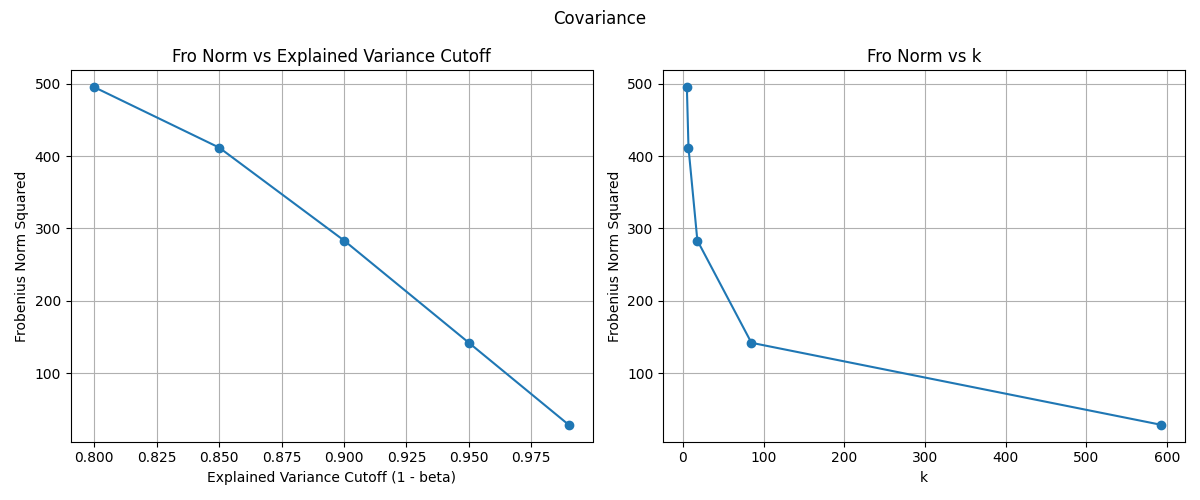
\includegraphics[width=\textwidth]{plots/OD_256_FrobeniusNormSquared_Covariance.png}
    \caption{\textbf{Frobenius Norm Squared vs $\beta$, OD $256\times256$, Covariance.}}
    \label{fig:fronorm_od256_cov}
\end{figure}

\begin{figure}[H]
    \centering
    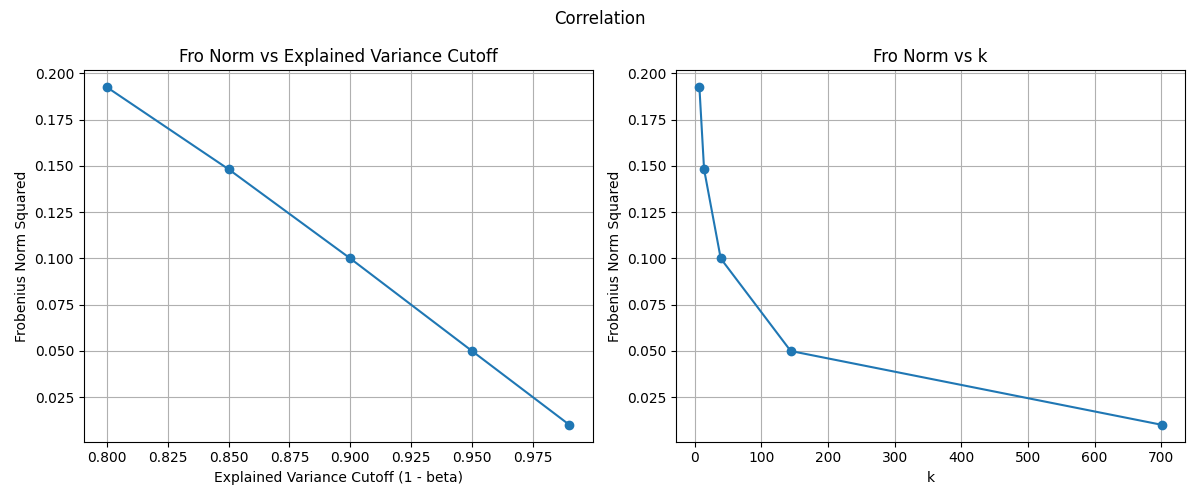
\includegraphics[width=\textwidth]{plots/OD_256_FrobeniusNormSquared_Correlation.png}
    \caption{\textbf{Frobenius Norm Squared vs $\beta$, OD $256\times256$, Correlation.}}
    \label{fig:fronorm_od256_cor}
\end{figure}

\begin{table*}[t]
\centering
\small
\begin{subtable}{0.32\linewidth}
\centering
\caption{RAW Reconstruction}
\begin{tabular}{cccc}
\hline
Metric & $\beta=0.01$ & $\beta=0.05$ & $\beta=0.1$ \\
\hline
MSE & 0.002606 & 0.006590 & 0.006590 \\
\hline
\end{tabular}
\end{subtable}
\hfill
\begin{subtable}{0.32\linewidth}
\centering
\caption{COV Reconstruction}
\begin{tabular}{cccc}
\hline
Metric & $\beta=0.01$ & $\beta=0.05$ & $\beta=0.1$ \\
\hline
MSE & 0.000145 & 0.000722 & 0.001442 \\
\hline
\end{tabular}
\end{subtable}
\hfill
\begin{subtable}{0.32\linewidth}
\centering
\caption{COR Reconstruction}
\begin{tabular}{cccc}
\hline
Metric & $\beta=0.01$ & $\beta=0.05$ & $\beta=0.1$ \\
\hline
MSE & 0.000139 & 0.000554 & 0.001072 \\
\hline
\end{tabular}
\end{subtable}
\caption{Average reconstruction MSE for different values of $\beta$ -- OD, $s=256$.}
\label{tab:mse_od_256}
\end{table*}

\begin{figure*}[t]
\centering
\begin{tabular}{cccc}
\textbf{Original} &
\textbf{$1-\beta = 0.99$} &
\textbf{$1-\beta = 0.95$} &
\textbf{$1-\beta = 0.90$} \\
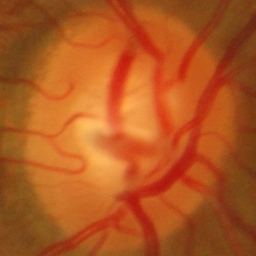
\includegraphics[width=0.22\linewidth]{images/OD_256_original_0.png} &
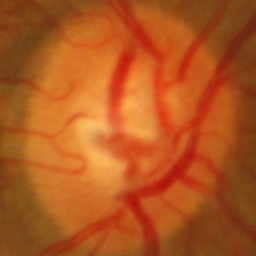
\includegraphics[width=0.22\linewidth]{images/OD_256_recon_cor_0_beta_99.png} &
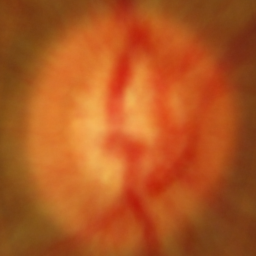
\includegraphics[width=0.22\linewidth]{images/OD_256_recon_cor_0_beta_95.png} &
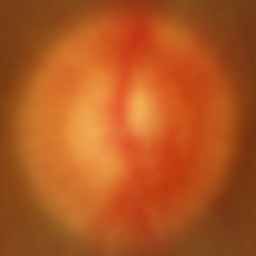
\includegraphics[width=0.22\linewidth]{images/OD_256_recon_cor_0_beta_90.png} \\
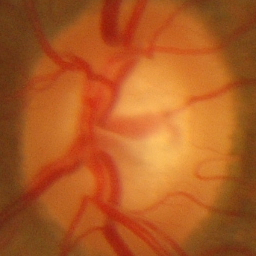
\includegraphics[width=0.22\linewidth]{images/OD_256_original_1.png} &
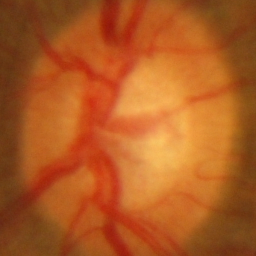
\includegraphics[width=0.22\linewidth]{images/OD_256_recon_cor_1_beta_99.png} &
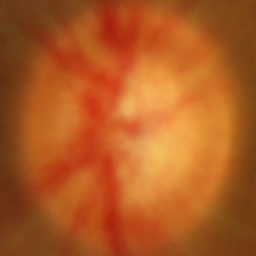
\includegraphics[width=0.22\linewidth]{images/OD_256_recon_cor_1_beta_95.png} &
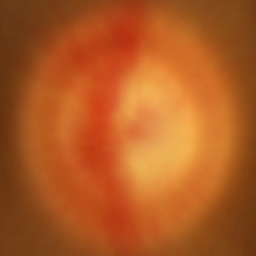
\includegraphics[width=0.22\linewidth]{images/OD_256_recon_cor_1_beta_90.png} \\
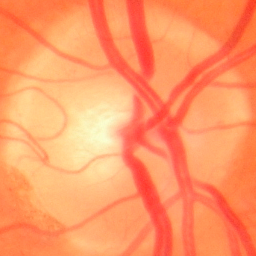
\includegraphics[width=0.22\linewidth]{images/OD_256_original_2.png} &
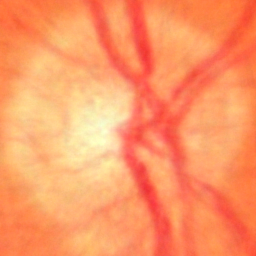
\includegraphics[width=0.22\linewidth]{images/OD_256_recon_cor_2_beta_99.png} &
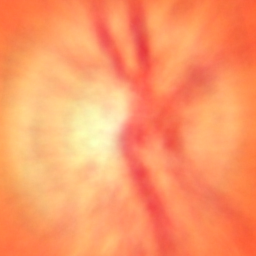
\includegraphics[width=0.22\linewidth]{images/OD_256_recon_cor_2_beta_95.png} &
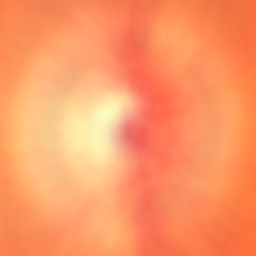
\includegraphics[width=0.22\linewidth]{images/OD_256_recon_cor_2_beta_90.png} \\
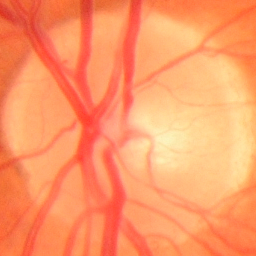
\includegraphics[width=0.22\linewidth]{images/OD_256_original_3.png} &
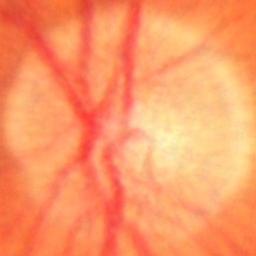
\includegraphics[width=0.22\linewidth]{images/OD_256_recon_cor_3_beta_99.png} &
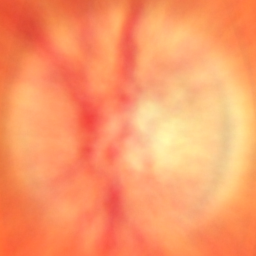
\includegraphics[width=0.22\linewidth]{images/OD_256_recon_cor_3_beta_95.png} &
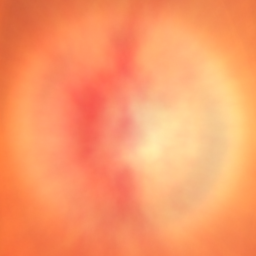
\includegraphics[width=0.22\linewidth]{images/OD_256_recon_cor_3_beta_90.png} \\
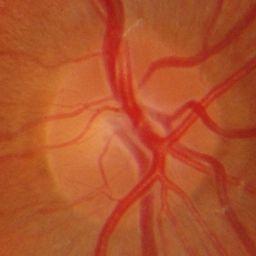
\includegraphics[width=0.22\linewidth]{images/OD_256_original_4.png} &
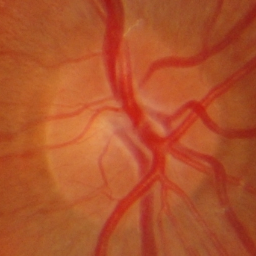
\includegraphics[width=0.22\linewidth]{images/OD_256_recon_cor_4_beta_99.png} &
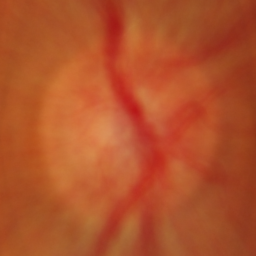
\includegraphics[width=0.22\linewidth]{images/OD_256_recon_cor_4_beta_95.png} &
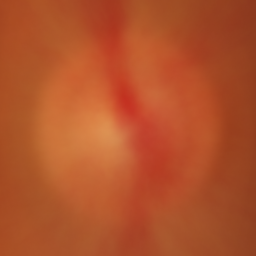
\includegraphics[width=0.22\linewidth]{images/OD_256_recon_cor_4_beta_90.png} \\
\end{tabular}
\caption{
Comparison of reconstructed OD crops ($s=256$) for different values of
$\beta$, using the \textbf{Correlation Analysis} basis. The leftmost column
shows the original crops.
}
\label{fig:reconstruction_grid_od256_cor}
\end{figure*}

\clearpage

% ============================================================
% OD 512
% ============================================================

\subsection{Optic Disc, $512\times512$}

\begin{table}[H]
    \centering
    \caption{Component Selection Summary -- OD, $s=512$}
    \label{tab:results_od_512}
    \vspace{0.2cm}
    \begin{tabular}{lrrrrr}
        \toprule
        \textbf{Analysis Type} & \textbf{$\beta$} & \textbf{Cutoff} & \textbf{Components Kept ($k$)} & \textbf{Actual Var. Expl.} & \textbf{Frobenius Norm} \\
        \midrule
        Raw Moments & 0.01 & 99.00\% & \textbf{9} & 99.06\% & 2759582.52\\
        Covariance  & 0.01 & 99.00\% & \textbf{747} & 99.00\% & 117.97 \\
        Correlation  & 0.01 & 99.00\% & \textbf{851} & 99.00\% & 0.01\\
        \bottomrule
    \end{tabular}
\end{table}

\begin{figure}[H]
    \centering
    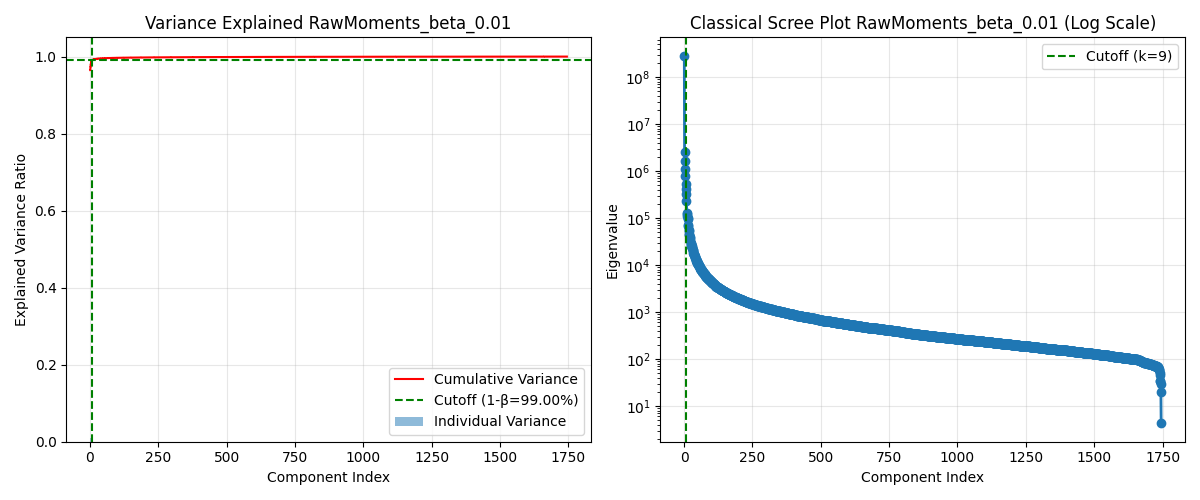
\includegraphics[width=\textwidth]{plots/OD_512_RawMoments_beta_0.01.png}
    \caption{\textbf{Raw Moments Analysis, OD $512\times512$.} Requires $k=9$ components.}
    \label{fig:od512_raw}
\end{figure}

\begin{figure}[H]
    \centering
    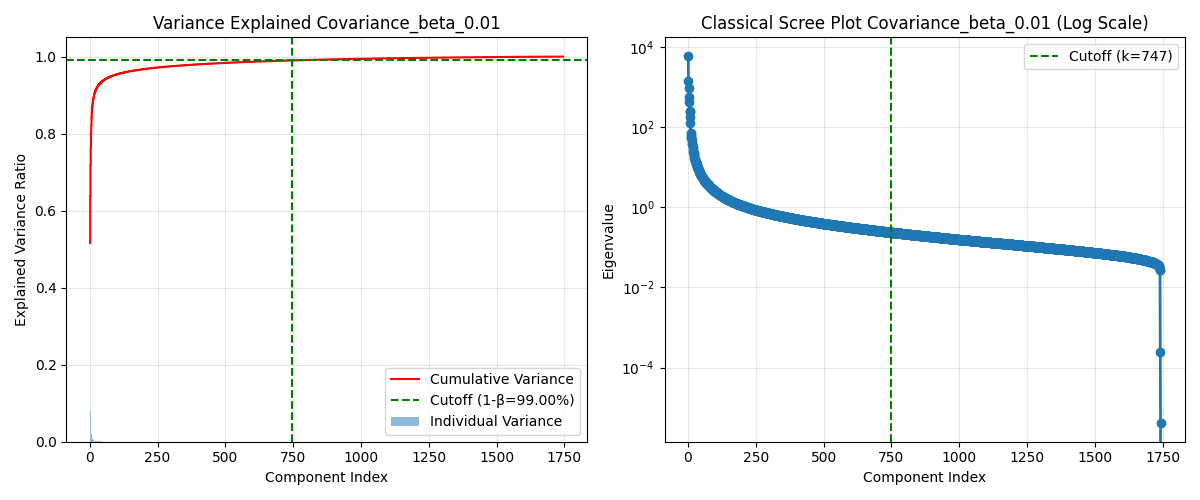
\includegraphics[width=\textwidth]{plots/OD_512_Covariance_beta_0.01.png}
    \caption{\textbf{Covariance Analysis (PCA), OD $512\times512$.} Requires $k=747$ components.}
    \label{fig:od512_cov}
\end{figure}

\begin{figure}[H]
    \centering
    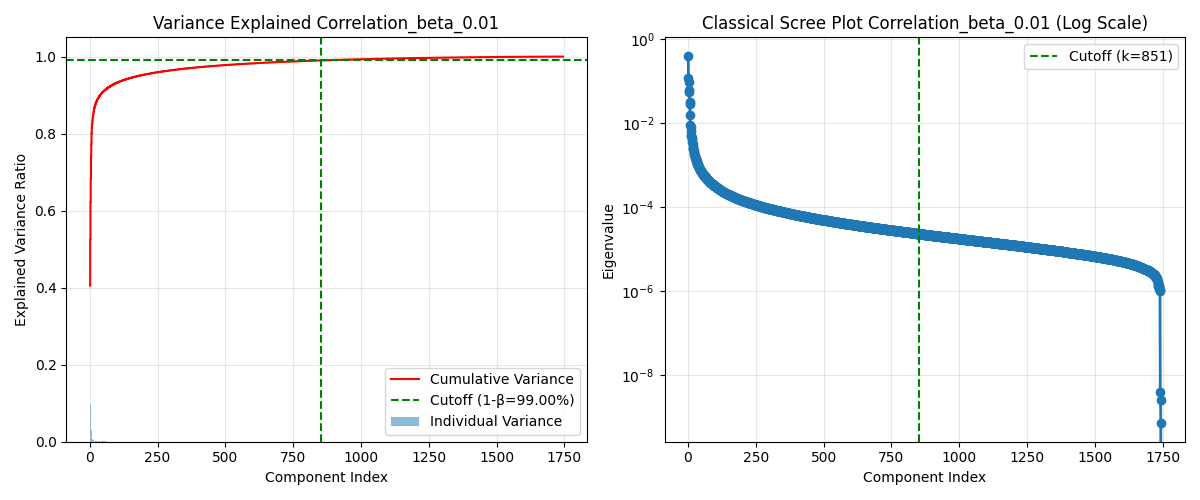
\includegraphics[width=\textwidth]{plots/OD_512_Correlation_beta_0.01.png}
    \caption{\textbf{Correlation Analysis, OD $512\times512$.} Requires $k=851$ components.}
    \label{fig:od512_cor}
\end{figure}

\begin{figure}[H]
    \centering
    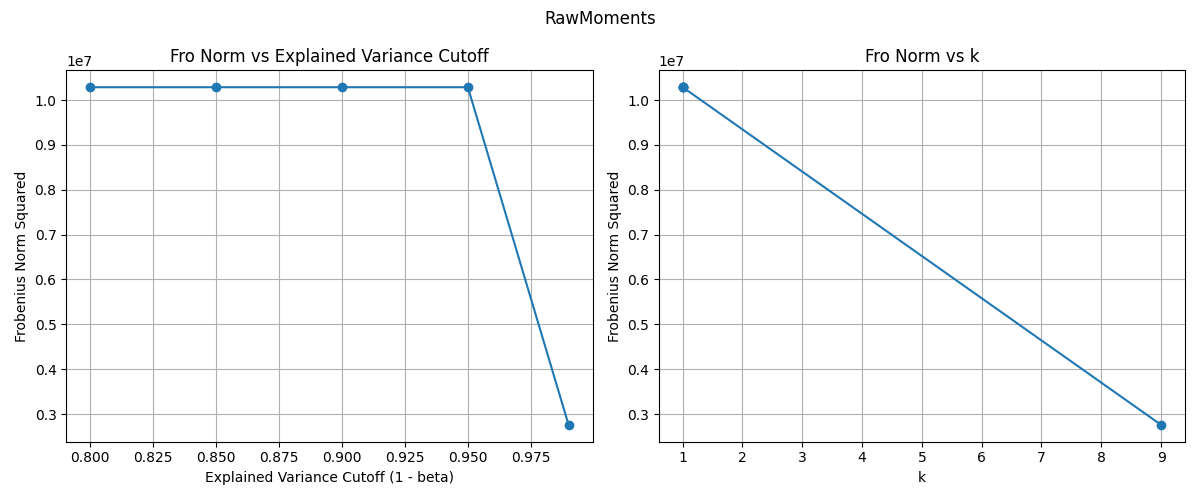
\includegraphics[width=\textwidth]{plots/OD_512_FrobeniusNormSquared_RawMoments.png}
    \caption{\textbf{Frobenius Norm Squared vs $\beta$, OD $512\times512$, Raw Moments.}}
    \label{fig:fronorm_od512_raw}
\end{figure}

\begin{figure}[H]
    \centering
    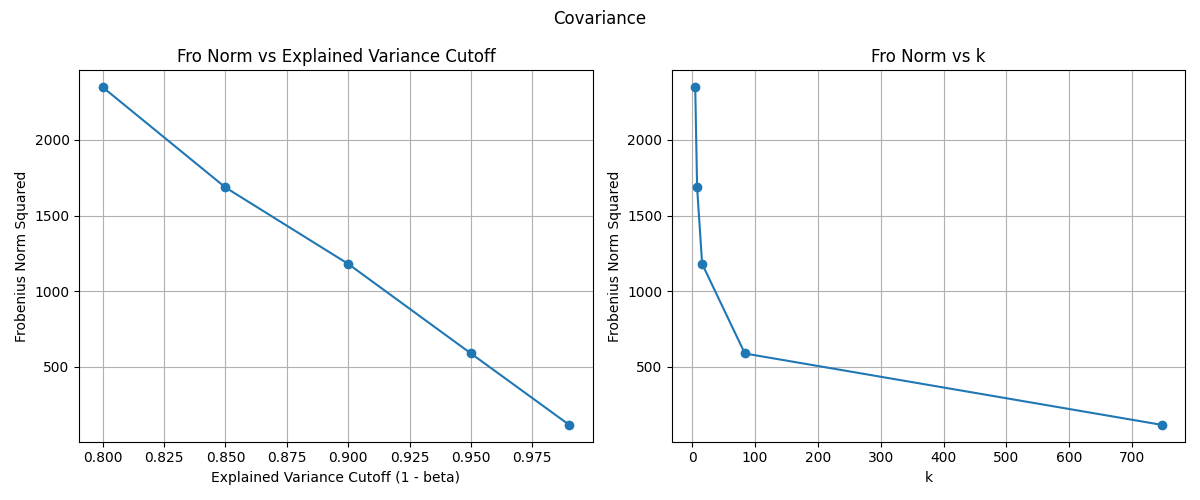
\includegraphics[width=\textwidth]{plots/OD_512_FrobeniusNormSquared_Covariance.png}
    \caption{\textbf{Frobenius Norm Squared vs $\beta$, OD $512\times512$, Covariance.}}
    \label{fig:fronorm_od512_cov}
\end{figure}

\begin{figure}[H]
    \centering
    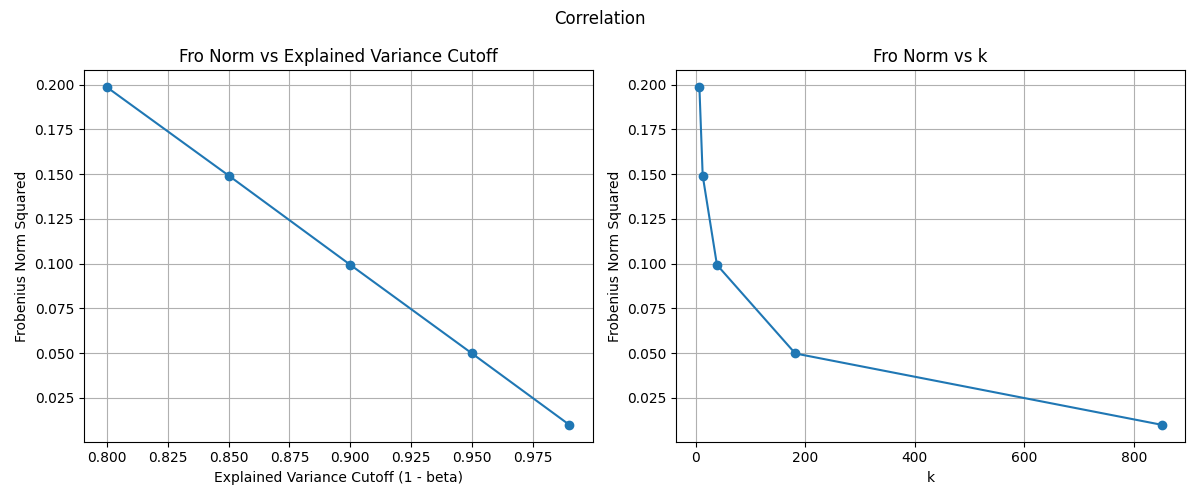
\includegraphics[width=\textwidth]{plots/OD_512_FrobeniusNormSquared_Correlation.png}
    \caption{\textbf{Frobenius Norm Squared vs $\beta$, OD $512\times512$, Correlation.}}
    \label{fig:fronorm_od512_cor}
\end{figure}

\begin{table*}[t]
\centering
\small
\begin{subtable}{0.32\linewidth}
\centering
\caption{RAW Reconstruction}
\begin{tabular}{cccc}
\hline
Metric & $\beta=0.01$ & $\beta=0.05$ & $\beta=0.1$ \\
\hline
MSE & 0.002015 & 0.007499 & 0.007499 \\
\hline
\end{tabular}
\end{subtable}
\hfill
\begin{subtable}{0.32\linewidth}
\centering
\caption{COV Reconstruction}
\begin{tabular}{cccc}
\hline
Metric & $\beta=0.01$ & $\beta=0.05$ & $\beta=0.1$ \\
\hline
MSE & 0.000150 & 0.000749 & 0.001501 \\
\hline
\end{tabular}
\end{subtable}
\hfill
\begin{subtable}{0.32\linewidth}
\centering
\caption{COR Reconstruction}
\begin{tabular}{cccc}
\hline
Metric & $\beta=0.01$ & $\beta=0.05$ & $\beta=0.1$ \\
\hline
MSE & 0.000163 & 0.000561 & 0.001068 \\
\hline
\end{tabular}
\end{subtable}
\caption{Average reconstruction MSE for different values of $\beta$ -- OD, $s=512$.}
\label{tab:mse_od_512}
\end{table*}

\begin{figure*}[t]
\centering
\begin{tabular}{cccc}
\textbf{Original} &
\textbf{$1-\beta = 0.99$} &
\textbf{$1-\beta = 0.95$} &
\textbf{$1-\beta = 0.90$} \\
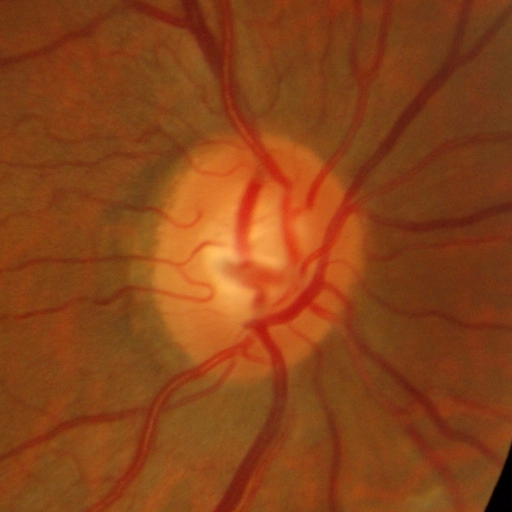
\includegraphics[width=0.22\linewidth]{images/OD_512_original_0.png} &
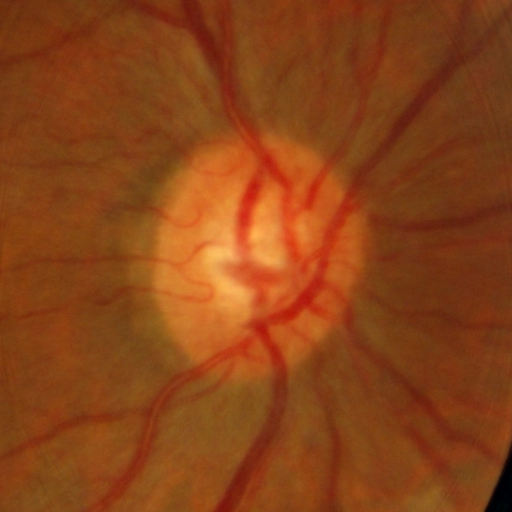
\includegraphics[width=0.22\linewidth]{images/OD_512_recon_cor_0_beta_99.png} &
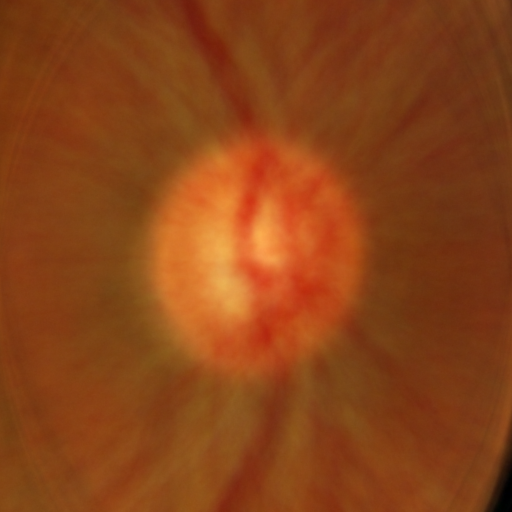
\includegraphics[width=0.22\linewidth]{images/OD_512_recon_cor_0_beta_95.png} &
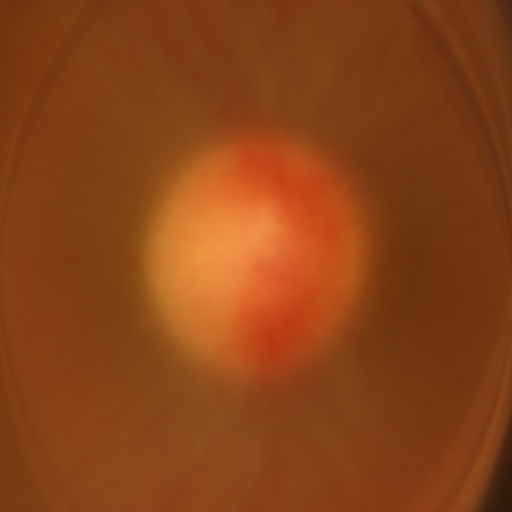
\includegraphics[width=0.22\linewidth]{images/OD_512_recon_cor_0_beta_90.png} \\
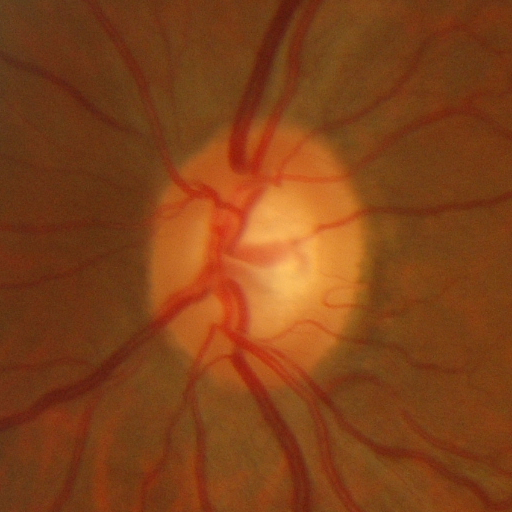
\includegraphics[width=0.22\linewidth]{images/OD_512_original_1.png} &
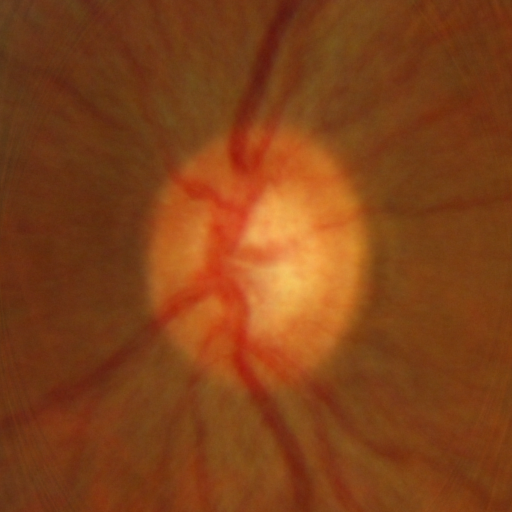
\includegraphics[width=0.22\linewidth]{images/OD_512_recon_cor_1_beta_99.png} &
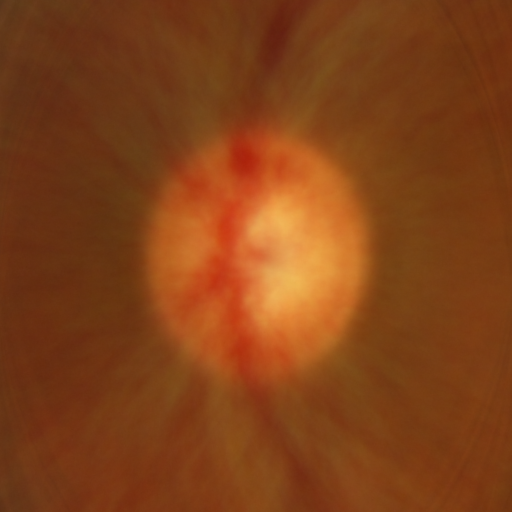
\includegraphics[width=0.22\linewidth]{images/OD_512_recon_cor_1_beta_95.png} &
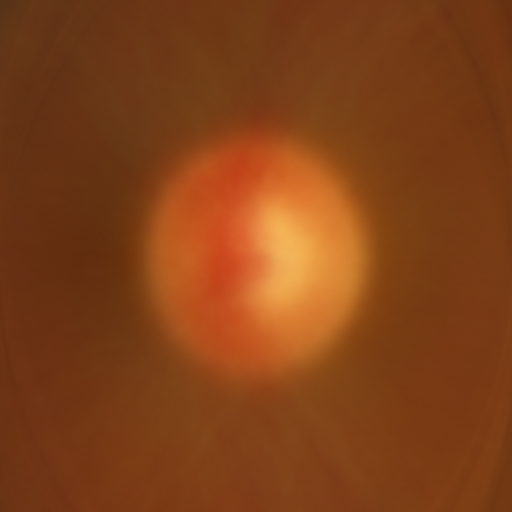
\includegraphics[width=0.22\linewidth]{images/OD_512_recon_cor_1_beta_90.png} \\
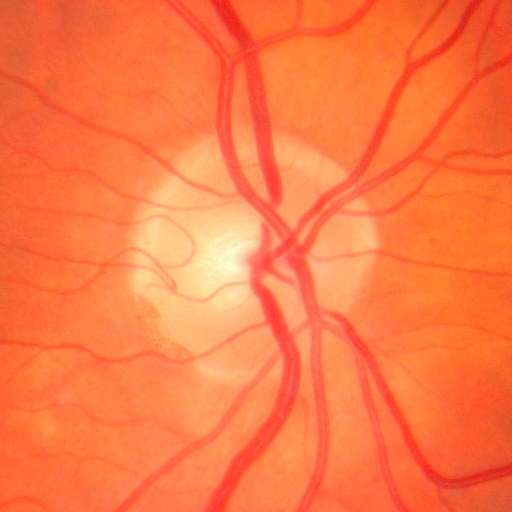
\includegraphics[width=0.22\linewidth]{images/OD_512_original_2.png} &
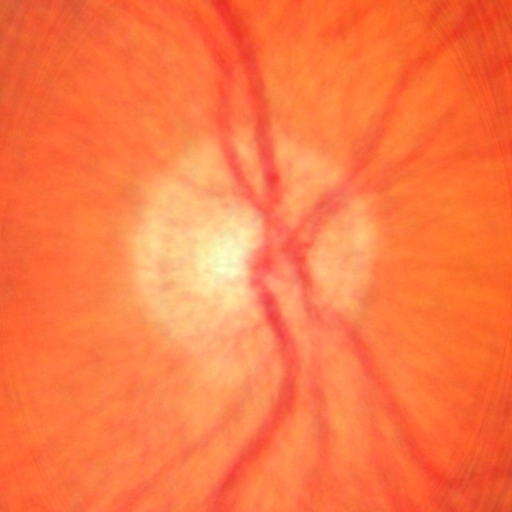
\includegraphics[width=0.22\linewidth]{images/OD_512_recon_cor_2_beta_99.png} &
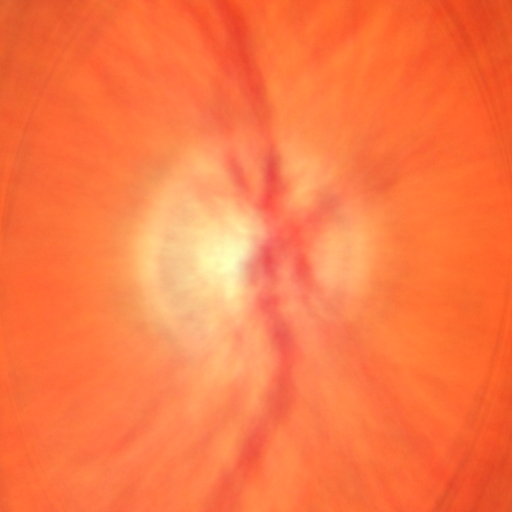
\includegraphics[width=0.22\linewidth]{images/OD_512_recon_cor_2_beta_95.png} &
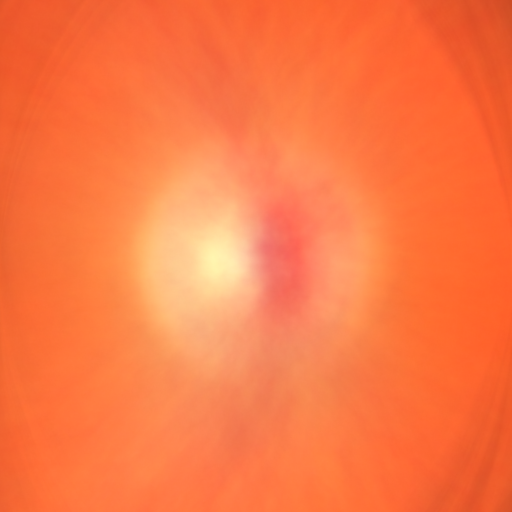
\includegraphics[width=0.22\linewidth]{images/OD_512_recon_cor_2_beta_90.png} \\
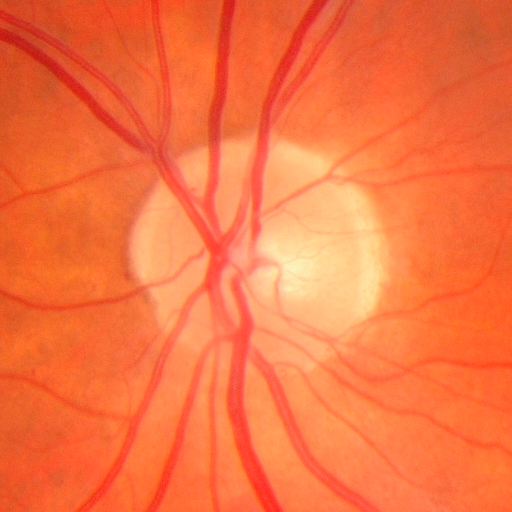
\includegraphics[width=0.22\linewidth]{images/OD_512_original_3.png} &
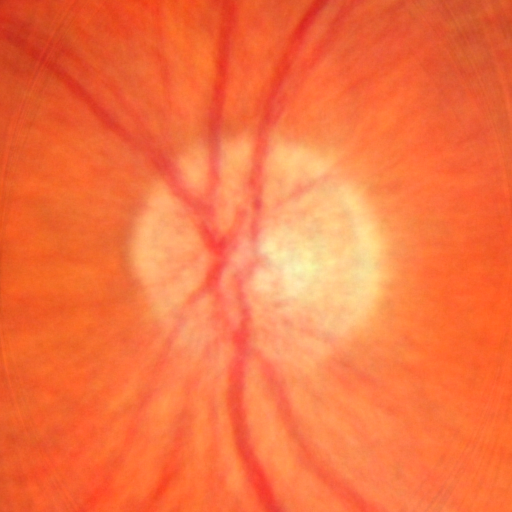
\includegraphics[width=0.22\linewidth]{images/OD_512_recon_cor_3_beta_99.png} &
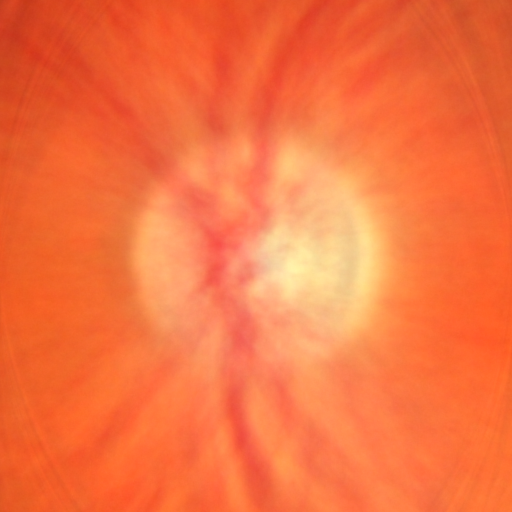
\includegraphics[width=0.22\linewidth]{images/OD_512_recon_cor_3_beta_95.png} &
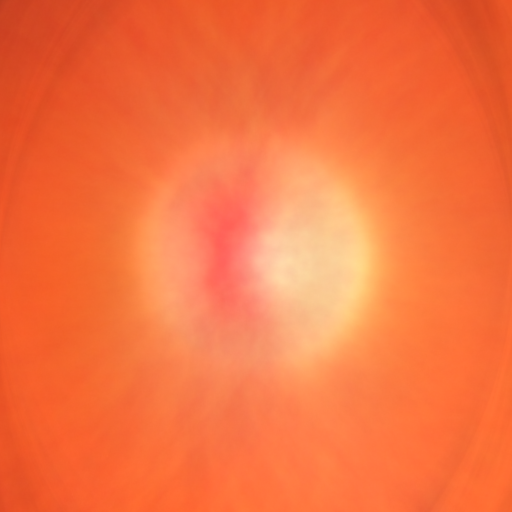
\includegraphics[width=0.22\linewidth]{images/OD_512_recon_cor_3_beta_90.png} \\
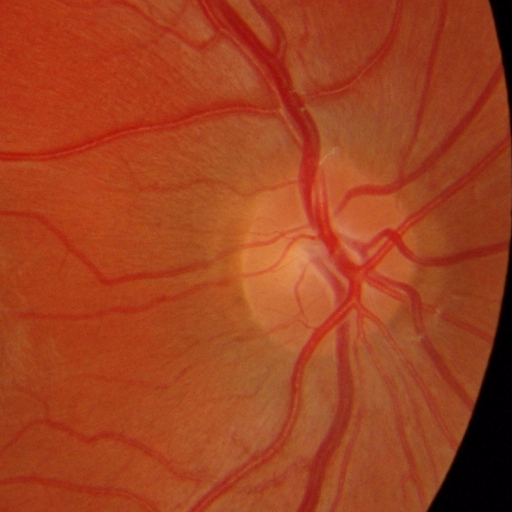
\includegraphics[width=0.22\linewidth]{images/OD_512_original_4.png} &
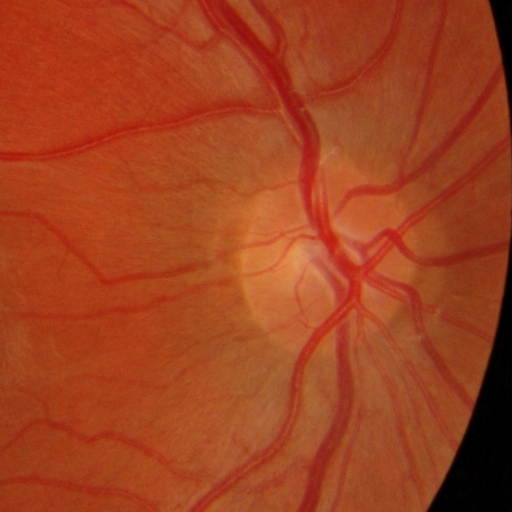
\includegraphics[width=0.22\linewidth]{images/OD_512_recon_cor_4_beta_99.png} &
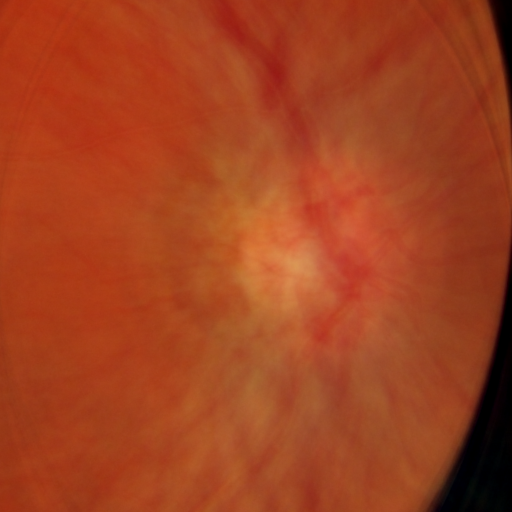
\includegraphics[width=0.22\linewidth]{images/OD_512_recon_cor_4_beta_95.png} &
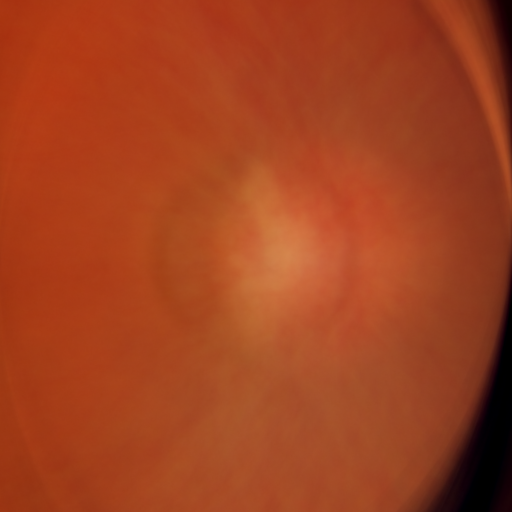
\includegraphics[width=0.22\linewidth]{images/OD_512_recon_cor_4_beta_90.png} \\
\end{tabular}
\caption{
Comparison of reconstructed OD crops ($s=512$) for different values of
$\beta$, using the \textbf{Correlation Analysis} basis. The leftmost column
shows the original crops.
}
\label{fig:reconstruction_grid_od512_cor}
\end{figure*}

\clearpage

% ============================================================
% FOVEA 256
% ============================================================

\subsection{Fovea, $256\times256$}

\begin{table}[H]
    \centering
    \caption{Component Selection Summary -- FOVEA, $s=256$}
    \label{tab:results_fovea_256}
    \vspace{0.2cm}
    \begin{tabular}{lrrrrr}
        \toprule
        \textbf{Analysis Type} & \textbf{$\beta$} & \textbf{Cutoff} & \textbf{Components Kept ($k$)} & \textbf{Actual Var. Expl.} & \textbf{Frobenius Norm} \\
        \midrule
        Raw Moments & 0.01 & 99.00\% & \textbf{2} & 99.25\% & 395471.86\\
        Covariance  & 0.01 & 99.00\% & \textbf{160} & 99.00\% & 22.69 \\
        Correlation  & 0.01 & 99.00\% & \textbf{469} & 99.00\% & 0.01\\
        \bottomrule
    \end{tabular}
\end{table}

\begin{figure}[H]
    \centering
    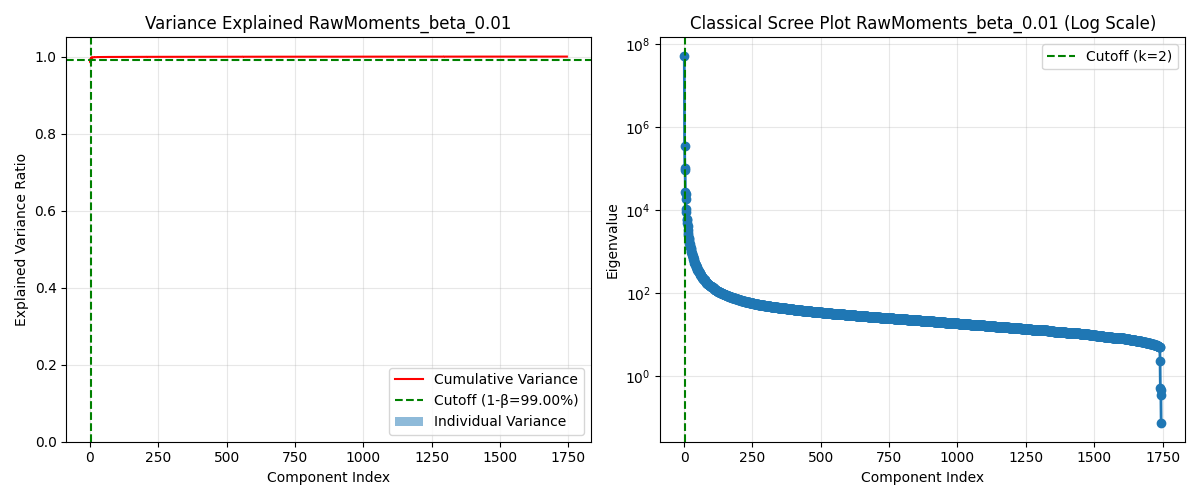
\includegraphics[width=\textwidth]{plots/FOVEA_256_RawMoments_beta_0.01.png}
    \caption{\textbf{Raw Moments Analysis, FOVEA $256\times256$.} Requires $k=2$ components.}
    \label{fig:fovea256_raw}
\end{figure}

\begin{figure}[H]
    \centering
    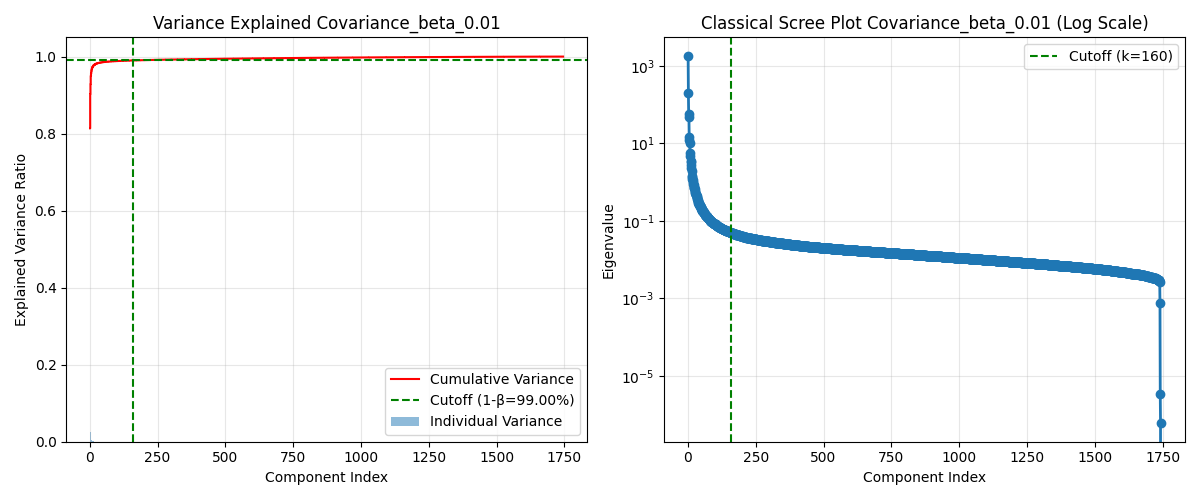
\includegraphics[width=\textwidth]{plots/FOVEA_256_Covariance_beta_0.01.png}
    \caption{\textbf{Covariance Analysis (PCA), FOVEA $256\times256$.} Requires $k=160$ components.}
    \label{fig:fovea256_cov}
\end{figure}

\begin{figure}[H]
    \centering
    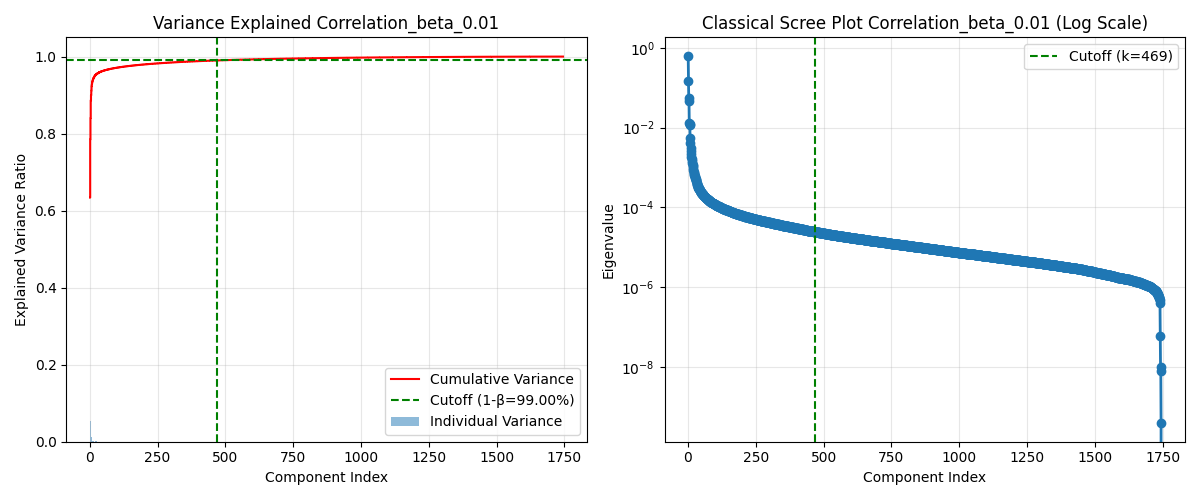
\includegraphics[width=\textwidth]{plots/FOVEA_256_Correlation_beta_0.01.png}
    \caption{\textbf{Correlation Analysis, FOVEA $256\times256$.} Requires $k=469$ components.}
    \label{fig:fovea256_cor}
\end{figure}

\begin{figure}[H]
    \centering
    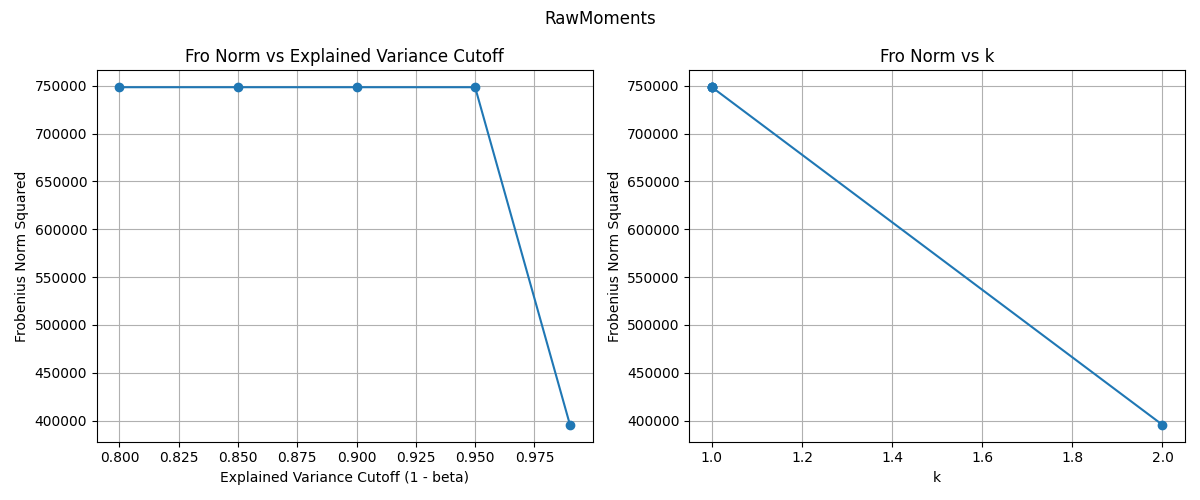
\includegraphics[width=\textwidth]{plots/FOVEA_256_FrobeniusNormSquared_RawMoments.png}
    \caption{\textbf{Frobenius Norm Squared vs $\beta$, FOVEA $256\times256$, Raw Moments.}}
    \label{fig:fronorm_fovea256_raw}
\end{figure}

\begin{figure}[H]
    \centering
    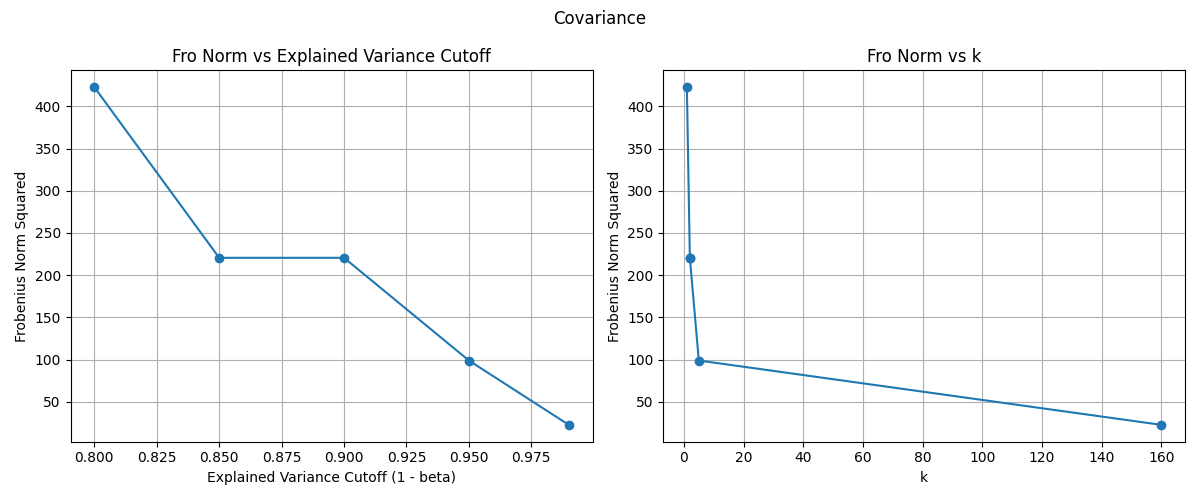
\includegraphics[width=\textwidth]{plots/FOVEA_256_FrobeniusNormSquared_Covariance.png}
    \caption{\textbf{Frobenius Norm Squared vs $\beta$, FOVEA $256\times256$, Covariance.}}
    \label{fig:fronorm_fovea256_cov}
\end{figure}

\begin{figure}[H]
    \centering
    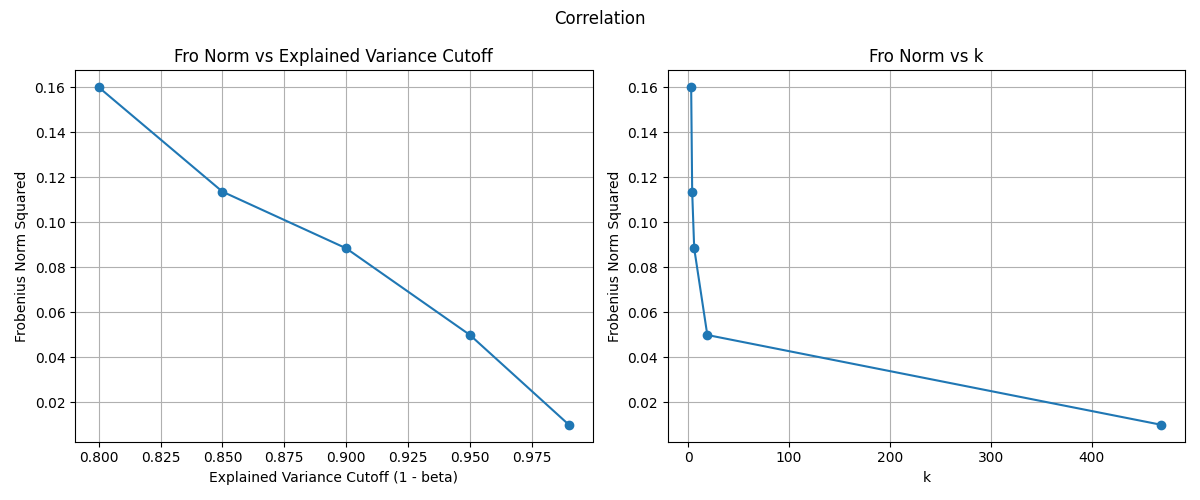
\includegraphics[width=\textwidth]{plots/FOVEA_256_FrobeniusNormSquared_Correlation.png}
    \caption{\textbf{Frobenius Norm Squared vs $\beta$, FOVEA $256\times256$, Correlation.}}
    \label{fig:fronorm_fovea256_cor}
\end{figure}

\begin{table*}[t]
\centering
\small
\begin{subtable}{0.32\linewidth}
\centering
\caption{RAW Reconstruction}
\begin{tabular}{cccc}
\hline
Metric & $\beta=0.01$ & $\beta=0.05$ & $\beta=0.1$ \\
\hline
MSE & 0.001158 & 0.002187 & 0.002187 \\
\hline
\end{tabular}
\end{subtable}
\hfill
\begin{subtable}{0.32\linewidth}
\centering
\caption{COV Reconstruction}
\begin{tabular}{cccc}
\hline
Metric & $\beta=0.01$ & $\beta=0.05$ & $\beta=0.1$ \\
\hline
MSE & 0.000116 & 0.000504 & 0.001122 \\
\hline
\end{tabular}
\end{subtable}
\hfill
\begin{subtable}{0.32\linewidth}
\centering
\caption{COR Reconstruction}
\begin{tabular}{cccc}
\hline
Metric & $\beta=0.01$ & $\beta=0.05$ & $\beta=0.1$ \\
\hline
MSE & 0.000090 & 0.000247 & 0.000455 \\
\hline
\end{tabular}
\end{subtable}
\caption{Average reconstruction MSE for different values of $\beta$ -- FOVEA, $s=256$.}
\label{tab:mse_fovea_256}
\end{table*}

\begin{figure*}[t]
\centering
\begin{tabular}{cccc}
\textbf{Original} &
\textbf{$1-\beta = 0.99$} &
\textbf{$1-\beta = 0.95$} &
\textbf{$1-\beta = 0.90$} \\
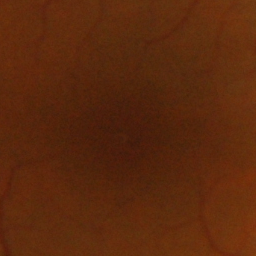
\includegraphics[width=0.22\linewidth]{images/FOVEA_256_original_0.png} &

\includegraphics[width=0.22\linewidth]{images/FOVEA_256_recon_cor_0_beta_99.png} &

\includegraphics[width=0.22\linewidth]{images/FOVEA_256_recon_cor_0_beta_95.png} &

\includegraphics[width=0.22\linewidth]{images/FOVEA_256_recon_cor_0_beta_90.png} \\
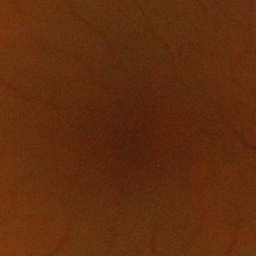
\includegraphics[width=0.22\linewidth]{images/FOVEA_256_original_1.png} &

\includegraphics[width=0.22\linewidth]{images/FOVEA_256_recon_cor_1_beta_99.png} &

\includegraphics[width=0.22\linewidth]{images/FOVEA_256_recon_cor_1_beta_95.png} &

\includegraphics[width=0.22\linewidth]{images/FOVEA_256_recon_cor_1_beta_90.png} \\
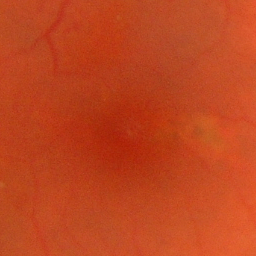
\includegraphics[width=0.22\linewidth]{images/FOVEA_256_original_2.png} &
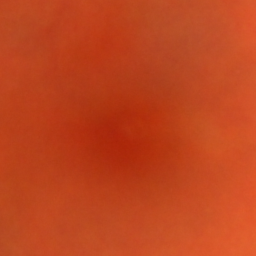
\includegraphics[width=0.22\linewidth]{images/FOVEA_256_recon_cor_2_beta_99.png} &

\includegraphics[width=0.22\linewidth]{images/FOVEA_256_recon_cor_2_beta_95.png} &

\includegraphics[width=0.22\linewidth]{images/FOVEA_256_recon_cor_2_beta_90.png} \\
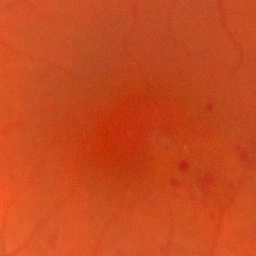
\includegraphics[width=0.22\linewidth]{images/FOVEA_256_original_3.png} &
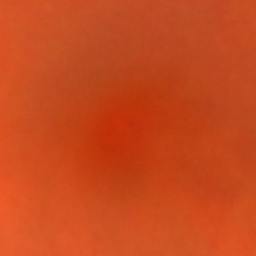
\includegraphics[width=0.22\linewidth]{images/FOVEA_256_recon_cor_3_beta_99.png} &

\includegraphics[width=0.22\linewidth]{images/FOVEA_256_recon_cor_3_beta_95.png} &

\includegraphics[width=0.22\linewidth]{images/FOVEA_256_recon_cor_3_beta_90.png} \\
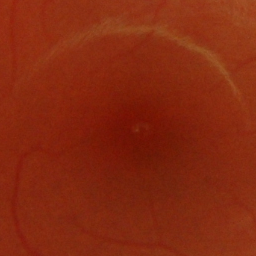
\includegraphics[width=0.22\linewidth]{images/FOVEA_256_original_4.png} &
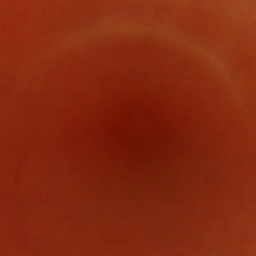
\includegraphics[width=0.22\linewidth]{images/FOVEA_256_recon_cor_4_beta_99.png} &

\includegraphics[width=0.22\linewidth]{images/FOVEA_256_recon_cor_4_beta_95.png} &

\includegraphics[width=0.22\linewidth]{images/FOVEA_256_recon_cor_4_beta_90.png} \\
\end{tabular}
\caption{
Comparison of reconstructed FOVEA crops ($s=256$) for different values of
$\beta$, using the \textbf{Correlation Analysis} basis. The leftmost column
shows the original crops.
}
\label{fig:reconstruction_grid_fovea256_cor}
\end{figure*}

\clearpage

% ============================================================
% FOVEA 512
% ============================================================

\subsection{Fovea, $512\times512$}

\begin{table}[H]
    \centering
    \caption{Component Selection Summary -- FOVEA, $s=512$}
    \label{tab:results_fovea_512}
    \vspace{0.2cm}
    \begin{tabular}{lrrrrr}
        \toprule
        \textbf{Analysis Type} & \textbf{$\beta$} & \textbf{Cutoff} & \textbf{Components Kept ($k$)} & \textbf{Actual Var. Expl.} & \textbf{Frobenius Norm} \\
        \midrule
        Raw Moments & 0.01 & 99.00\% & \textbf{3} & 99.32\% & 1599660.53\\
        Covariance  & 0.01 & 99.00\% & \textbf{424} & 99.00\% & 95.45 \\
        Correlation  & 0.01 & 99.00\% & \textbf{645} & 99.00\% & 0.01\\
        \bottomrule
    \end{tabular}
\end{table}

\begin{figure}[H]
    \centering
    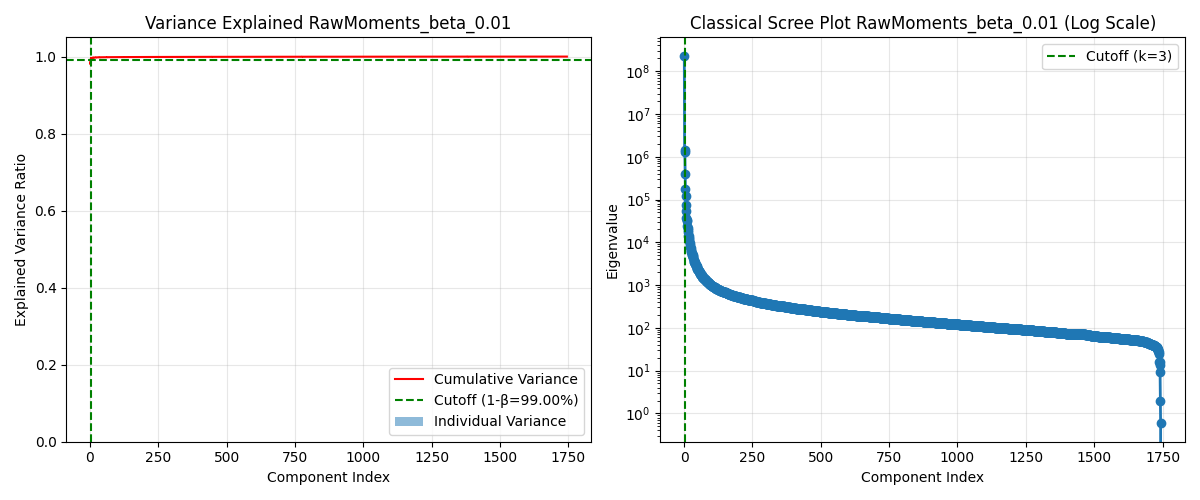
\includegraphics[width=\textwidth]{plots/FOVEA_512_RawMoments_beta_0.01.png}
    \caption{\textbf{Raw Moments Analysis, FOVEA $512\times512$.} Requires $k=3$ components.}
    \label{fig:fovea512_raw}
\end{figure}

\begin{figure}[H]
    \centering
    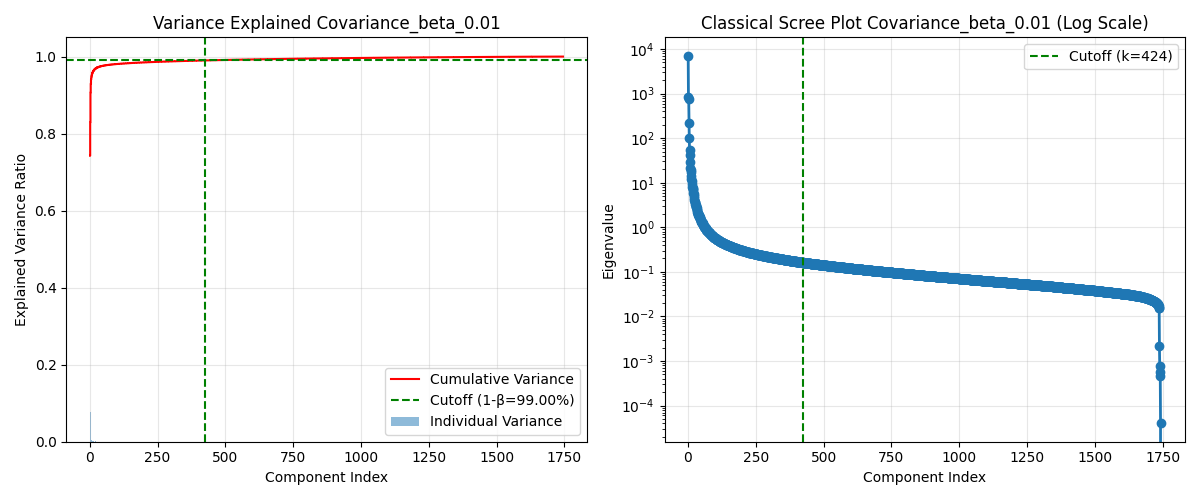
\includegraphics[width=\textwidth]{plots/FOVEA_512_Covariance_beta_0.01.png}
    \caption{\textbf{Covariance Analysis (PCA), FOVEA $512\times512$.} Requires $k=424$ components.}
    \label{fig:fovea512_cov}
\end{figure}

\begin{figure}[H]
    \centering
    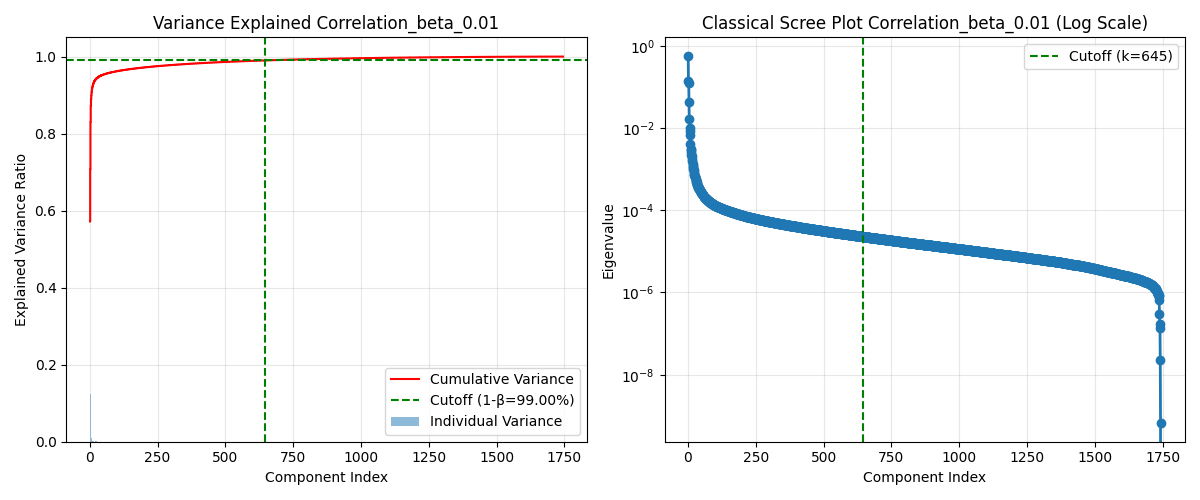
\includegraphics[width=\textwidth]{plots/FOVEA_512_Correlation_beta_0.01.png}
    \caption{\textbf{Correlation Analysis, FOVEA $512\times512$.} Requires $k=645$ components.}
    \label{fig:fovea512_cor}
\end{figure}

\begin{figure}[H]
    \centering
    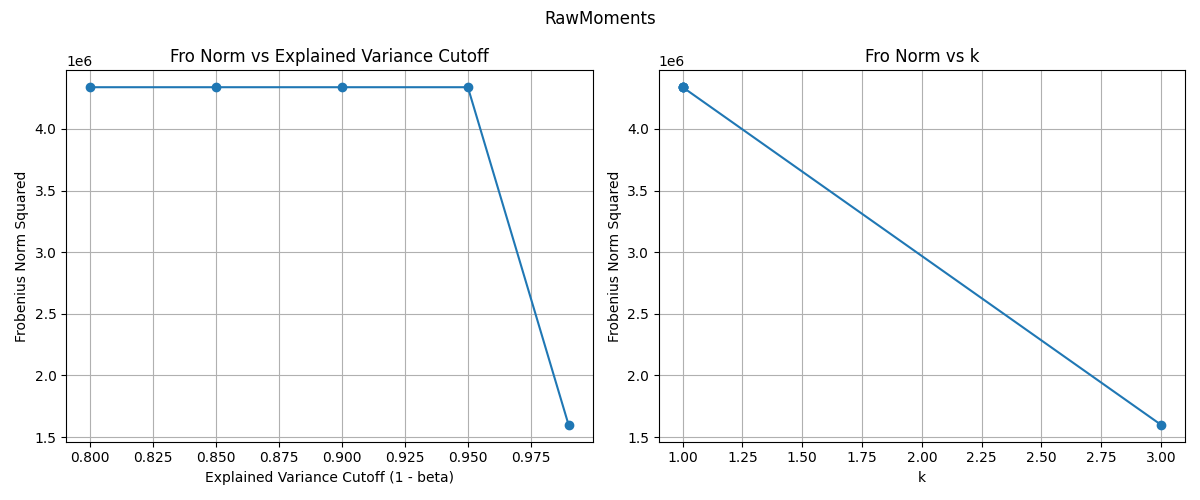
\includegraphics[width=\textwidth]{plots/FOVEA_512_FrobeniusNormSquared_RawMoments.png}
    \caption{\textbf{Frobenius Norm Squared vs $\beta$, FOVEA $512\times512$, Raw Moments.}}
    \label{fig:fronorm_fovea512_raw}
\end{figure}

\begin{figure}[H]
    \centering
    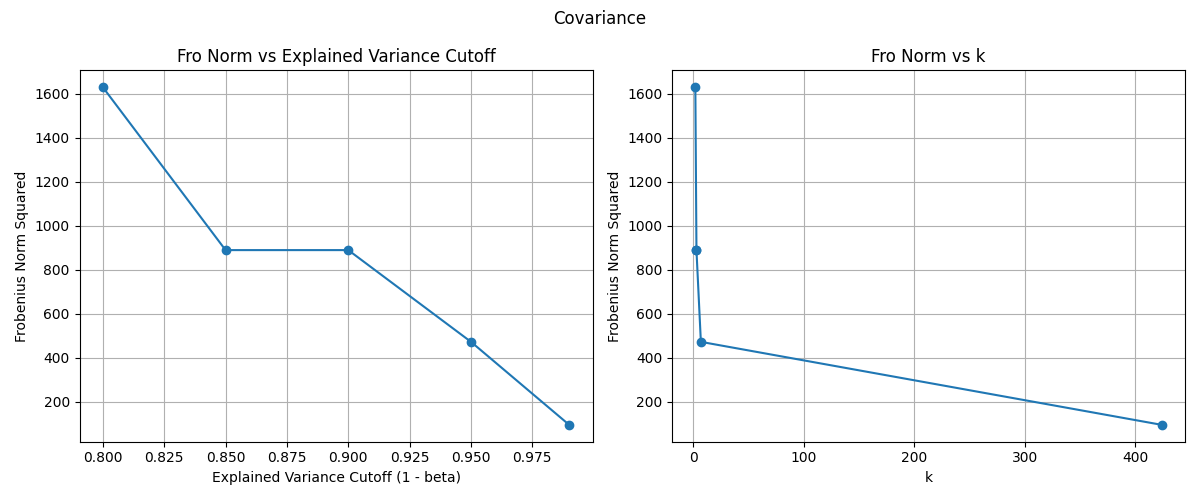
\includegraphics[width=\textwidth]{plots/FOVEA_512_FrobeniusNormSquared_Covariance.png}
    \caption{\textbf{Frobenius Norm Squared vs $\beta$, FOVEA $512\times512$, Covariance.}}
    \label{fig:fronorm_fovea512_cov}
\end{figure}

\begin{figure}[H]
    \centering
    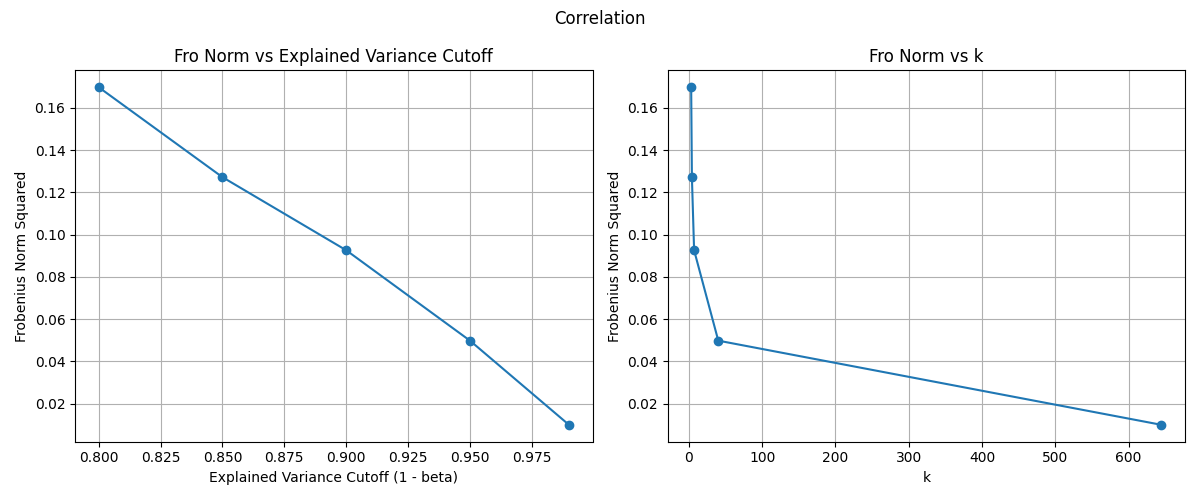
\includegraphics[width=\textwidth]{plots/FOVEA_512_FrobeniusNormSquared_Correlation.png}
    \caption{\textbf{Frobenius Norm Squared vs $\beta$, FOVEA $512\times512$, Correlation.}}
    \label{fig:fronorm_fovea512_cor}
\end{figure}

\begin{table*}[t]
\centering
\small
\begin{subtable}{0.32\linewidth}
\centering
\caption{RAW Reconstruction}
\begin{tabular}{cccc}
\hline
Metric & $\beta=0.01$ & $\beta=0.05$ & $\beta=0.1$ \\
\hline
MSE & 0.001170 & 0.003165 & 0.003165 \\
\hline
\end{tabular}
\end{subtable}
\hfill
\begin{subtable}{0.32\linewidth}
\centering
\caption{COV Reconstruction}
\begin{tabular}{cccc}
\hline
Metric & $\beta=0.01$ & $\beta=0.05$ & $\beta=0.1$ \\
\hline
MSE & 0.000122 & 0.000600 & 0.001130 \\
\hline
\end{tabular}
\end{subtable}
\hfill
\begin{subtable}{0.32\linewidth}
\centering
\caption{COR Reconstruction}
\begin{tabular}{cccc}
\hline
Metric & $\beta=0.01$ & $\beta=0.05$ & $\beta=0.1$ \\
\hline
MSE & 0.000117 & 0.000320 & 0.000608 \\
\hline
\end{tabular}
\end{subtable}
\caption{Average reconstruction MSE for different values of $\beta$ -- FOVEA, $s=512$.}
\label{tab:mse_fovea_512}
\end{table*}

\begin{figure*}[t]
\centering
\begin{tabular}{cccc}
\textbf{Original} &
\textbf{$1-\beta = 0.99$} &
\textbf{$1-\beta = 0.95$} &
\textbf{$1-\beta = 0.90$} \\
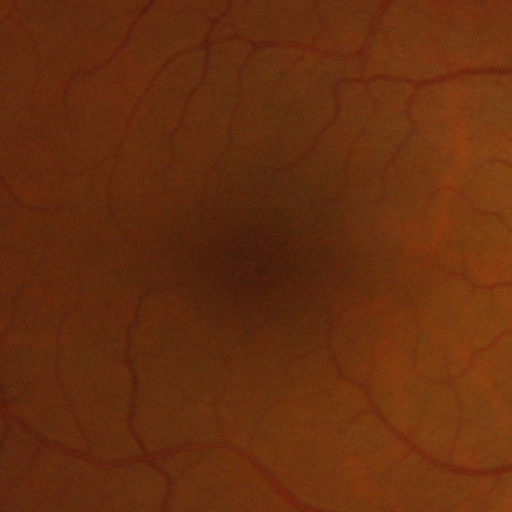
\includegraphics[width=0.22\linewidth]{images/FOVEA_512_original_0.png} &
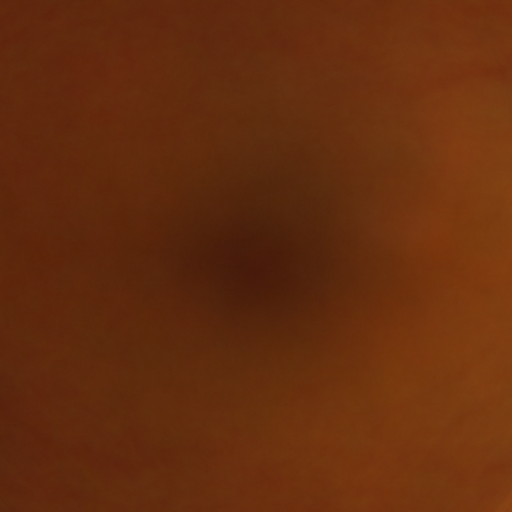
\includegraphics[width=0.22\linewidth]{images/FOVEA_512_recon_cor_0_beta_99.png} &
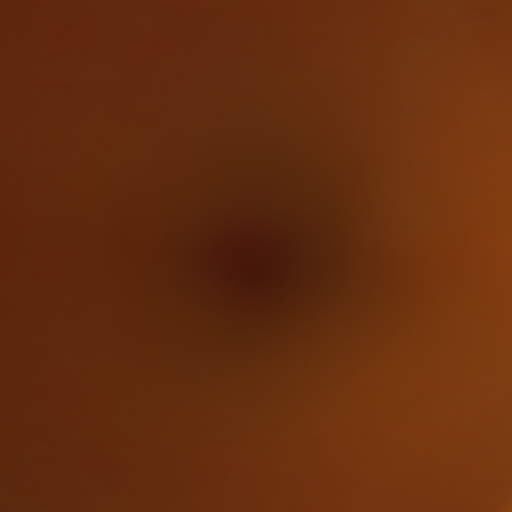
\includegraphics[width=0.22\linewidth]{images/FOVEA_512_recon_cor_0_beta_95.png} &

\includegraphics[width=0.22\linewidth]{images/FOVEA_512_recon_cor_0_beta_90.png} \\
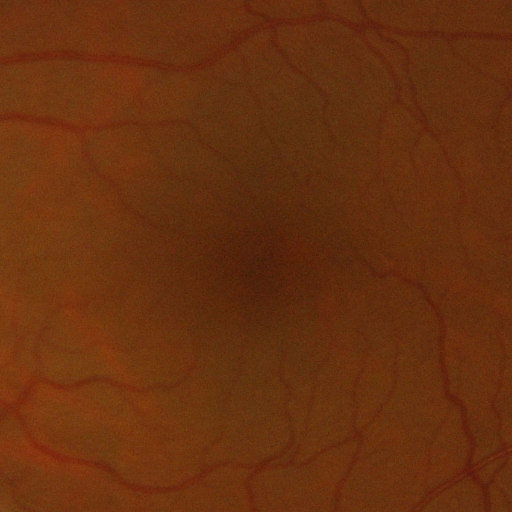
\includegraphics[width=0.22\linewidth]{images/FOVEA_512_original_1.png} &
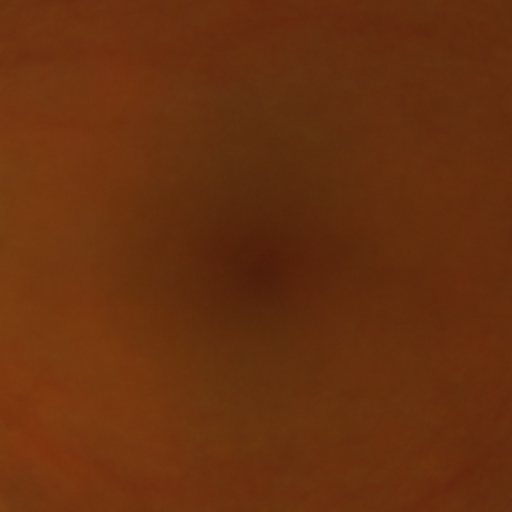
\includegraphics[width=0.22\linewidth]{images/FOVEA_512_recon_cor_1_beta_99.png} &

\includegraphics[width=0.22\linewidth]{images/FOVEA_512_recon_cor_1_beta_95.png} &

\includegraphics[width=0.22\linewidth]{images/FOVEA_512_recon_cor_1_beta_90.png} \\
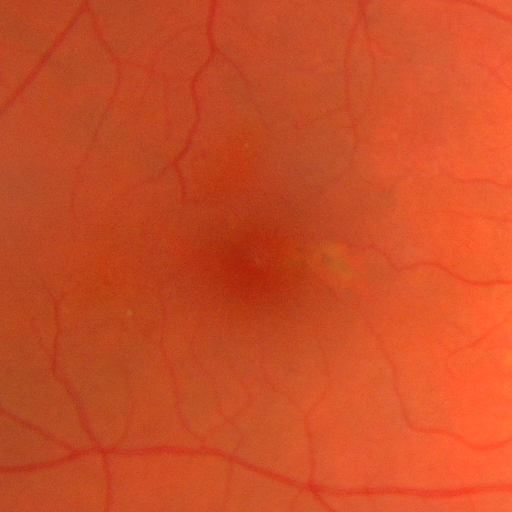
\includegraphics[width=0.22\linewidth]{images/FOVEA_512_original_2.png} &
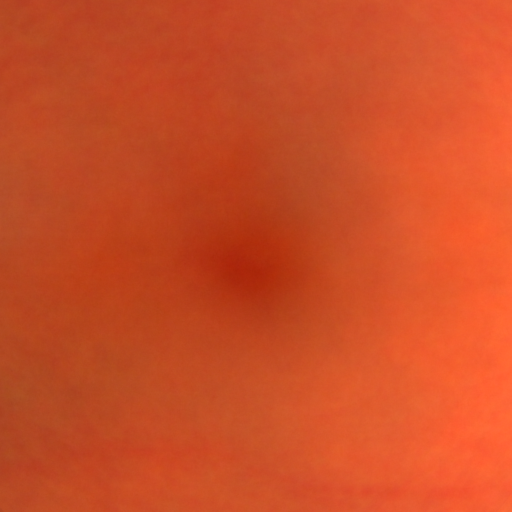
\includegraphics[width=0.22\linewidth]{images/FOVEA_512_recon_cor_2_beta_99.png} &
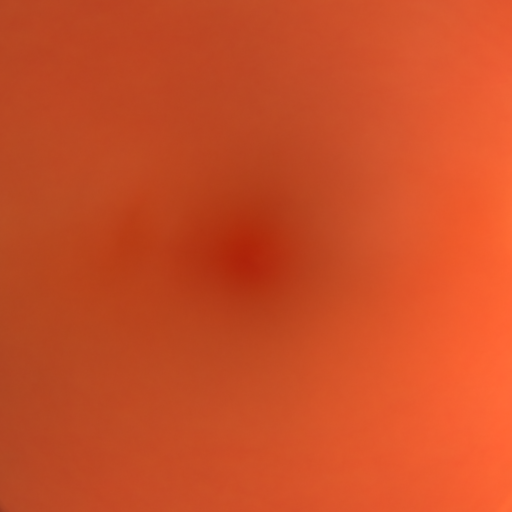
\includegraphics[width=0.22\linewidth]{images/FOVEA_512_recon_cor_2_beta_95.png} &

\includegraphics[width=0.22\linewidth]{images/FOVEA_512_recon_cor_2_beta_90.png} \\
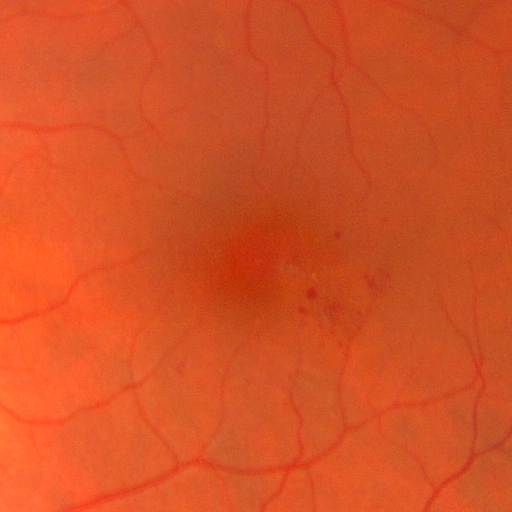
\includegraphics[width=0.22\linewidth]{images/FOVEA_512_original_3.png} &
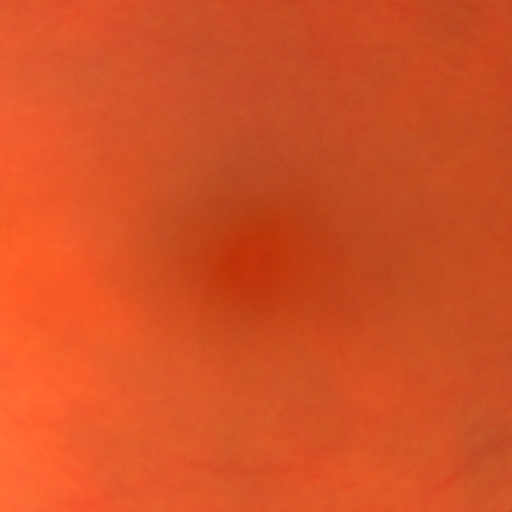
\includegraphics[width=0.22\linewidth]{images/FOVEA_512_recon_cor_3_beta_99.png} &
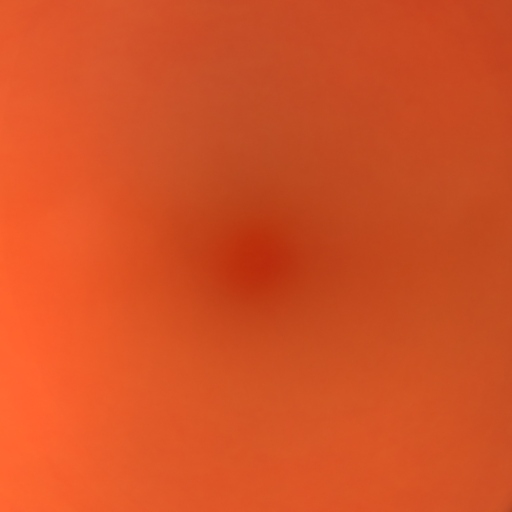
\includegraphics[width=0.22\linewidth]{images/FOVEA_512_recon_cor_3_beta_95.png} &

\includegraphics[width=0.22\linewidth]{images/FOVEA_512_recon_cor_3_beta_90.png} \\
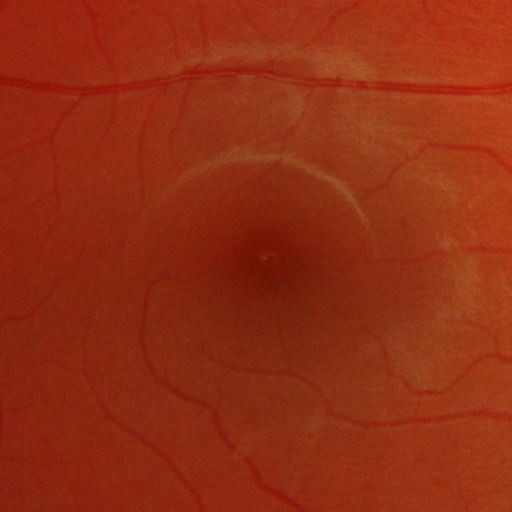
\includegraphics[width=0.22\linewidth]{images/FOVEA_512_original_4.png} &
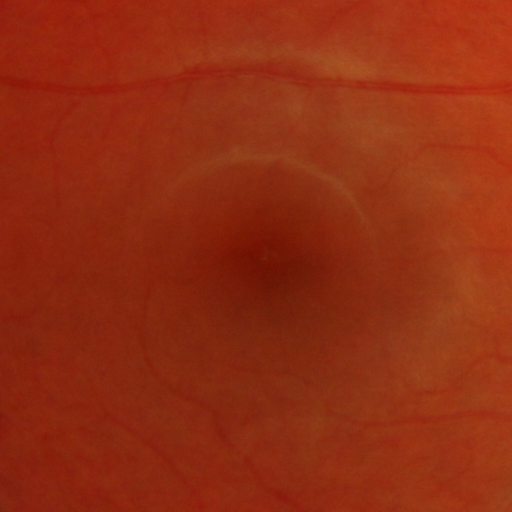
\includegraphics[width=0.22\linewidth]{images/FOVEA_512_recon_cor_4_beta_99.png} &

\includegraphics[width=0.22\linewidth]{images/FOVEA_512_recon_cor_4_beta_95.png} &

\includegraphics[width=0.22\linewidth]{images/FOVEA_512_recon_cor_4_beta_90.png} \\
\end{tabular}
\caption{
Comparison of reconstructed FOVEA crops ($s=512$) for different values of
$\beta$, using the \textbf{Correlation Analysis} basis. The leftmost column
shows the original crops.
}
\label{fig:reconstruction_grid_fovea512_cor}
\end{figure*}

\clearpage

\section{Conclusion}

Under Raw Moments, all four crop configurations need only a handful of
components ($k=5/9/2/3$ for OD 256/OD 512/FOVEA 256/FOVEA 512), since a
single mean-like direction dominates. Under Covariance and Correlation, the
OD crops need substantially more components than the FOVEA crops at matched
size ($k=593/701$ vs. $k=160/469$ for $s=256$; $k=747/851$ vs. $k=424/645$
for $s=512$) -- the optic disc's dense, image-specific vessel branching is
evidently less redundant than the visually more homogeneous fovea region.

On reconstruction quality, the Correlation-normalized basis gives the
lowest MSE in every configuration, followed by Covariance, with Raw Moments
consistently worst. MSE increases monotonically as $\beta$ increases (i.e.
as fewer components are kept),
without exception across all four crop configurations and all three
variants. FOVEA crops reconstruct more accurately than OD crops at matched
$\beta$ (e.g. FOVEA $256$/Cor/$\beta=0.01$: MSE $=0.000090$ vs. OD
$256$/Cor/$\beta=0.01$: MSE $=0.000139$), mirroring the same fovea/OD
homogeneity gap seen in the component-selection results above.

\end{document}
